\documentclass{article}
\usepackage{graphicx} % Required for inserting images
\usepackage{hyperref}
\usepackage[most]{tcolorbox}
\usepackage{caption}
\usepackage{subcaption}

\pgfkeysdef{/tcb/autowidth title}{
    \pgfmathwidth{"#1"}
    \def\width{\pgfmathresult pt} % \width = title length
%
    \tcbset{title=#1,
            tcbox width=minimum center,
            text width=\width % minimum text width = title length
           }
 }

\title{Assignment 5 Computation Creativity}
\author{Batch size of 3}
\date{November 2023}

\begin{document}

\maketitle

% 1. a clear description of the data collection, codebase/app, architecture, parameter choices, and tuning process. What additional code did you use/have to write? How long did it take to create the NeRF? What problems did you encounter and overcome? What did you learn that you would tell another student trying to do the same thing?

% 2. “bells and whistles”. Once you created the basic NeRF, what cool stuff were you able to do with it (e.g., cool renderings/camera paths/stylization)? What tools did you use for this part?

% 3. results and critical discussion. Are the results reasonable? What are some notable success and failure cases?

\section{\textbf{NOTE}: RESULTS ARE INCLUDED IN THE BOX FOLDER}

\section{NeRF}

\subsection{Data Acquisition}

We gathered three videos (shot by a phone) of different items in order to test the quality and effectiveness of the NeRF model that we will use.

\begin{center}
    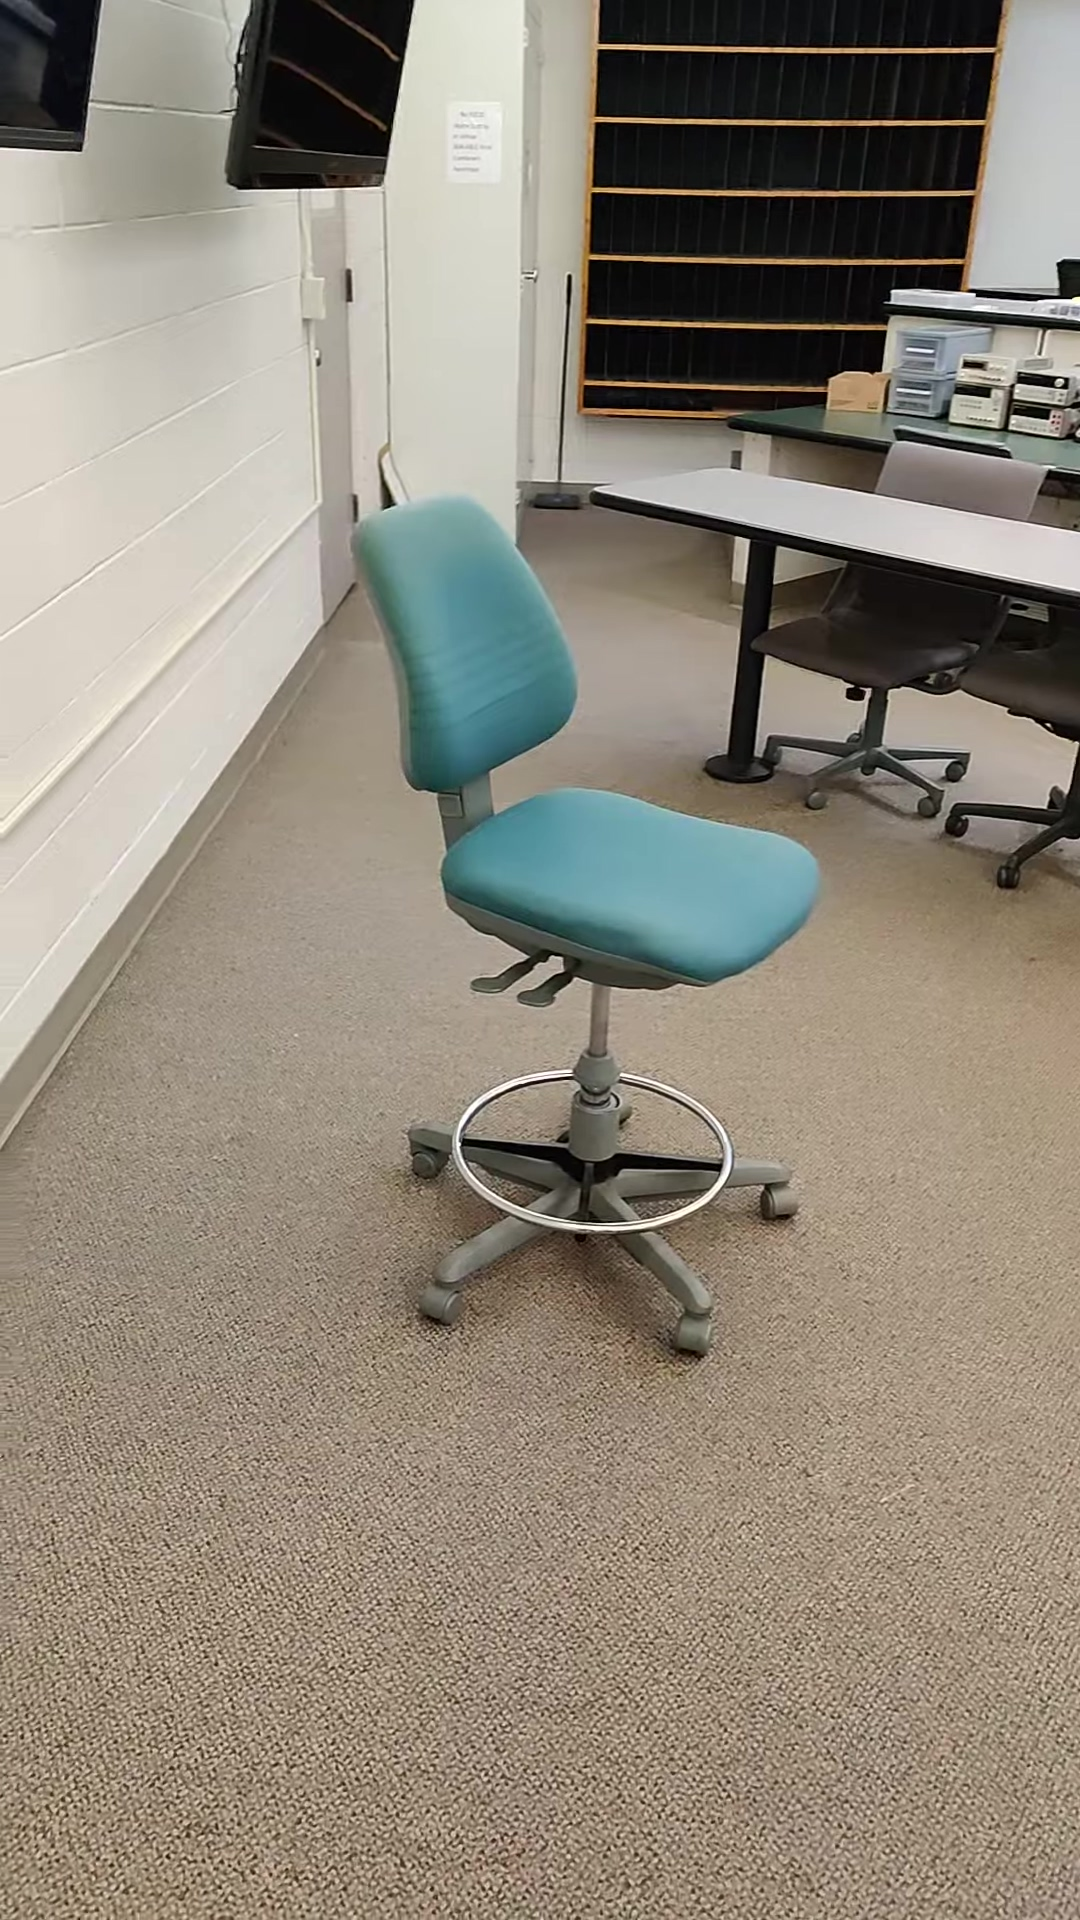
\includegraphics[scale=0.04]{images/chair1.jpg}
    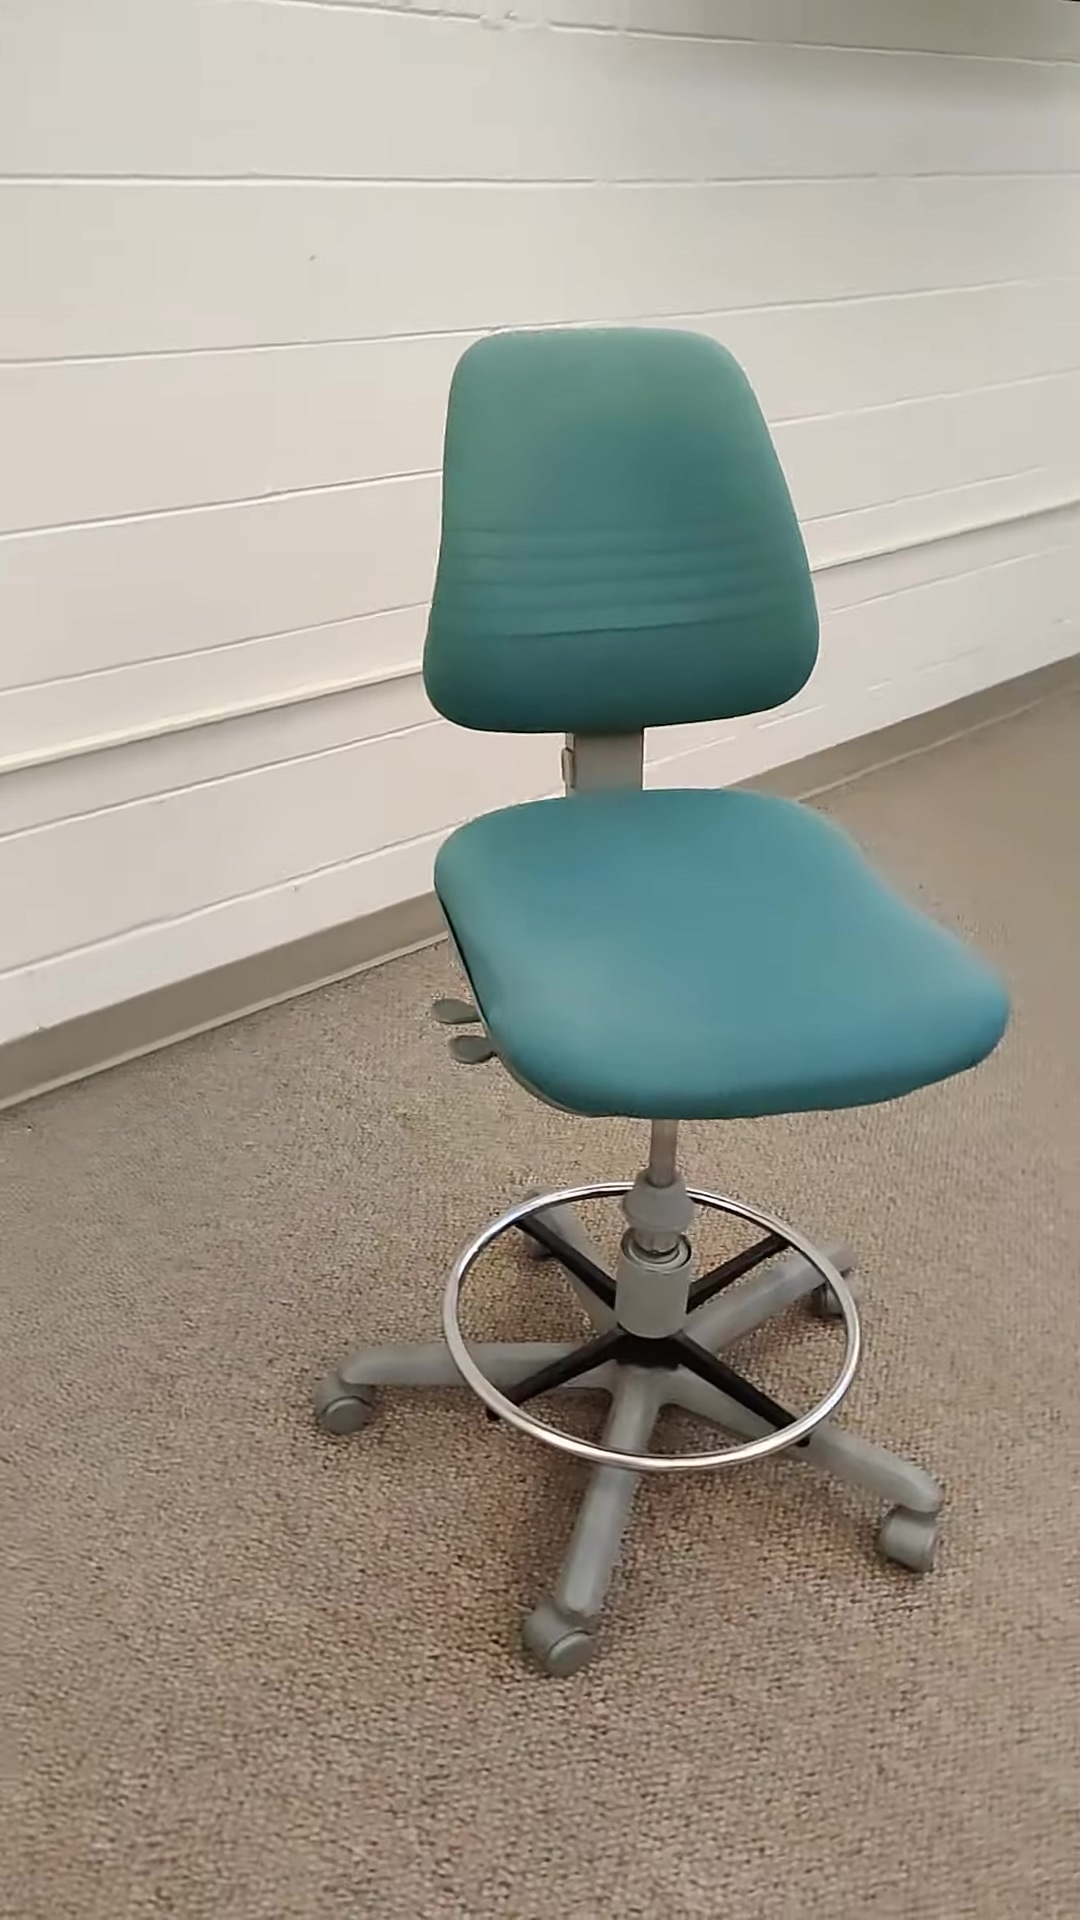
\includegraphics[scale=0.04]{images/chair2.jpg}
    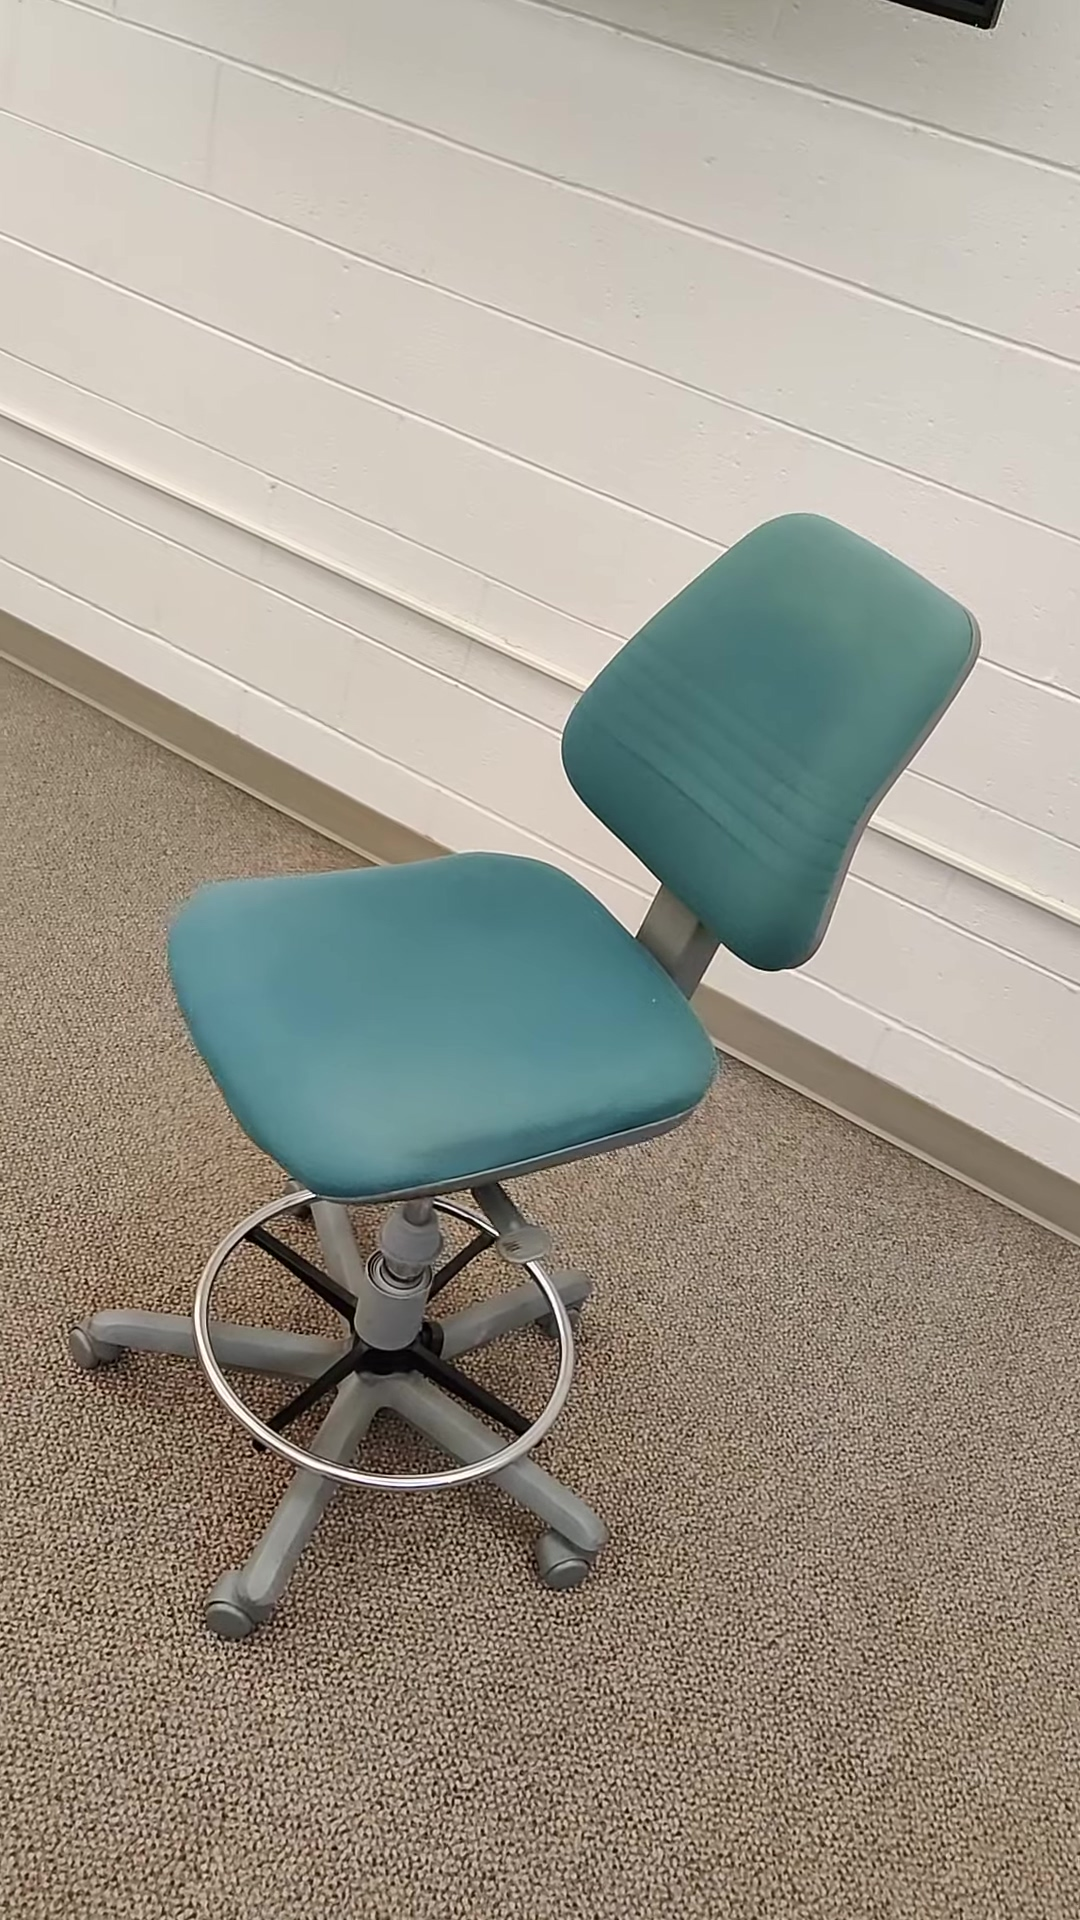
\includegraphics[scale=0.04]{images/chair3.jpg}
    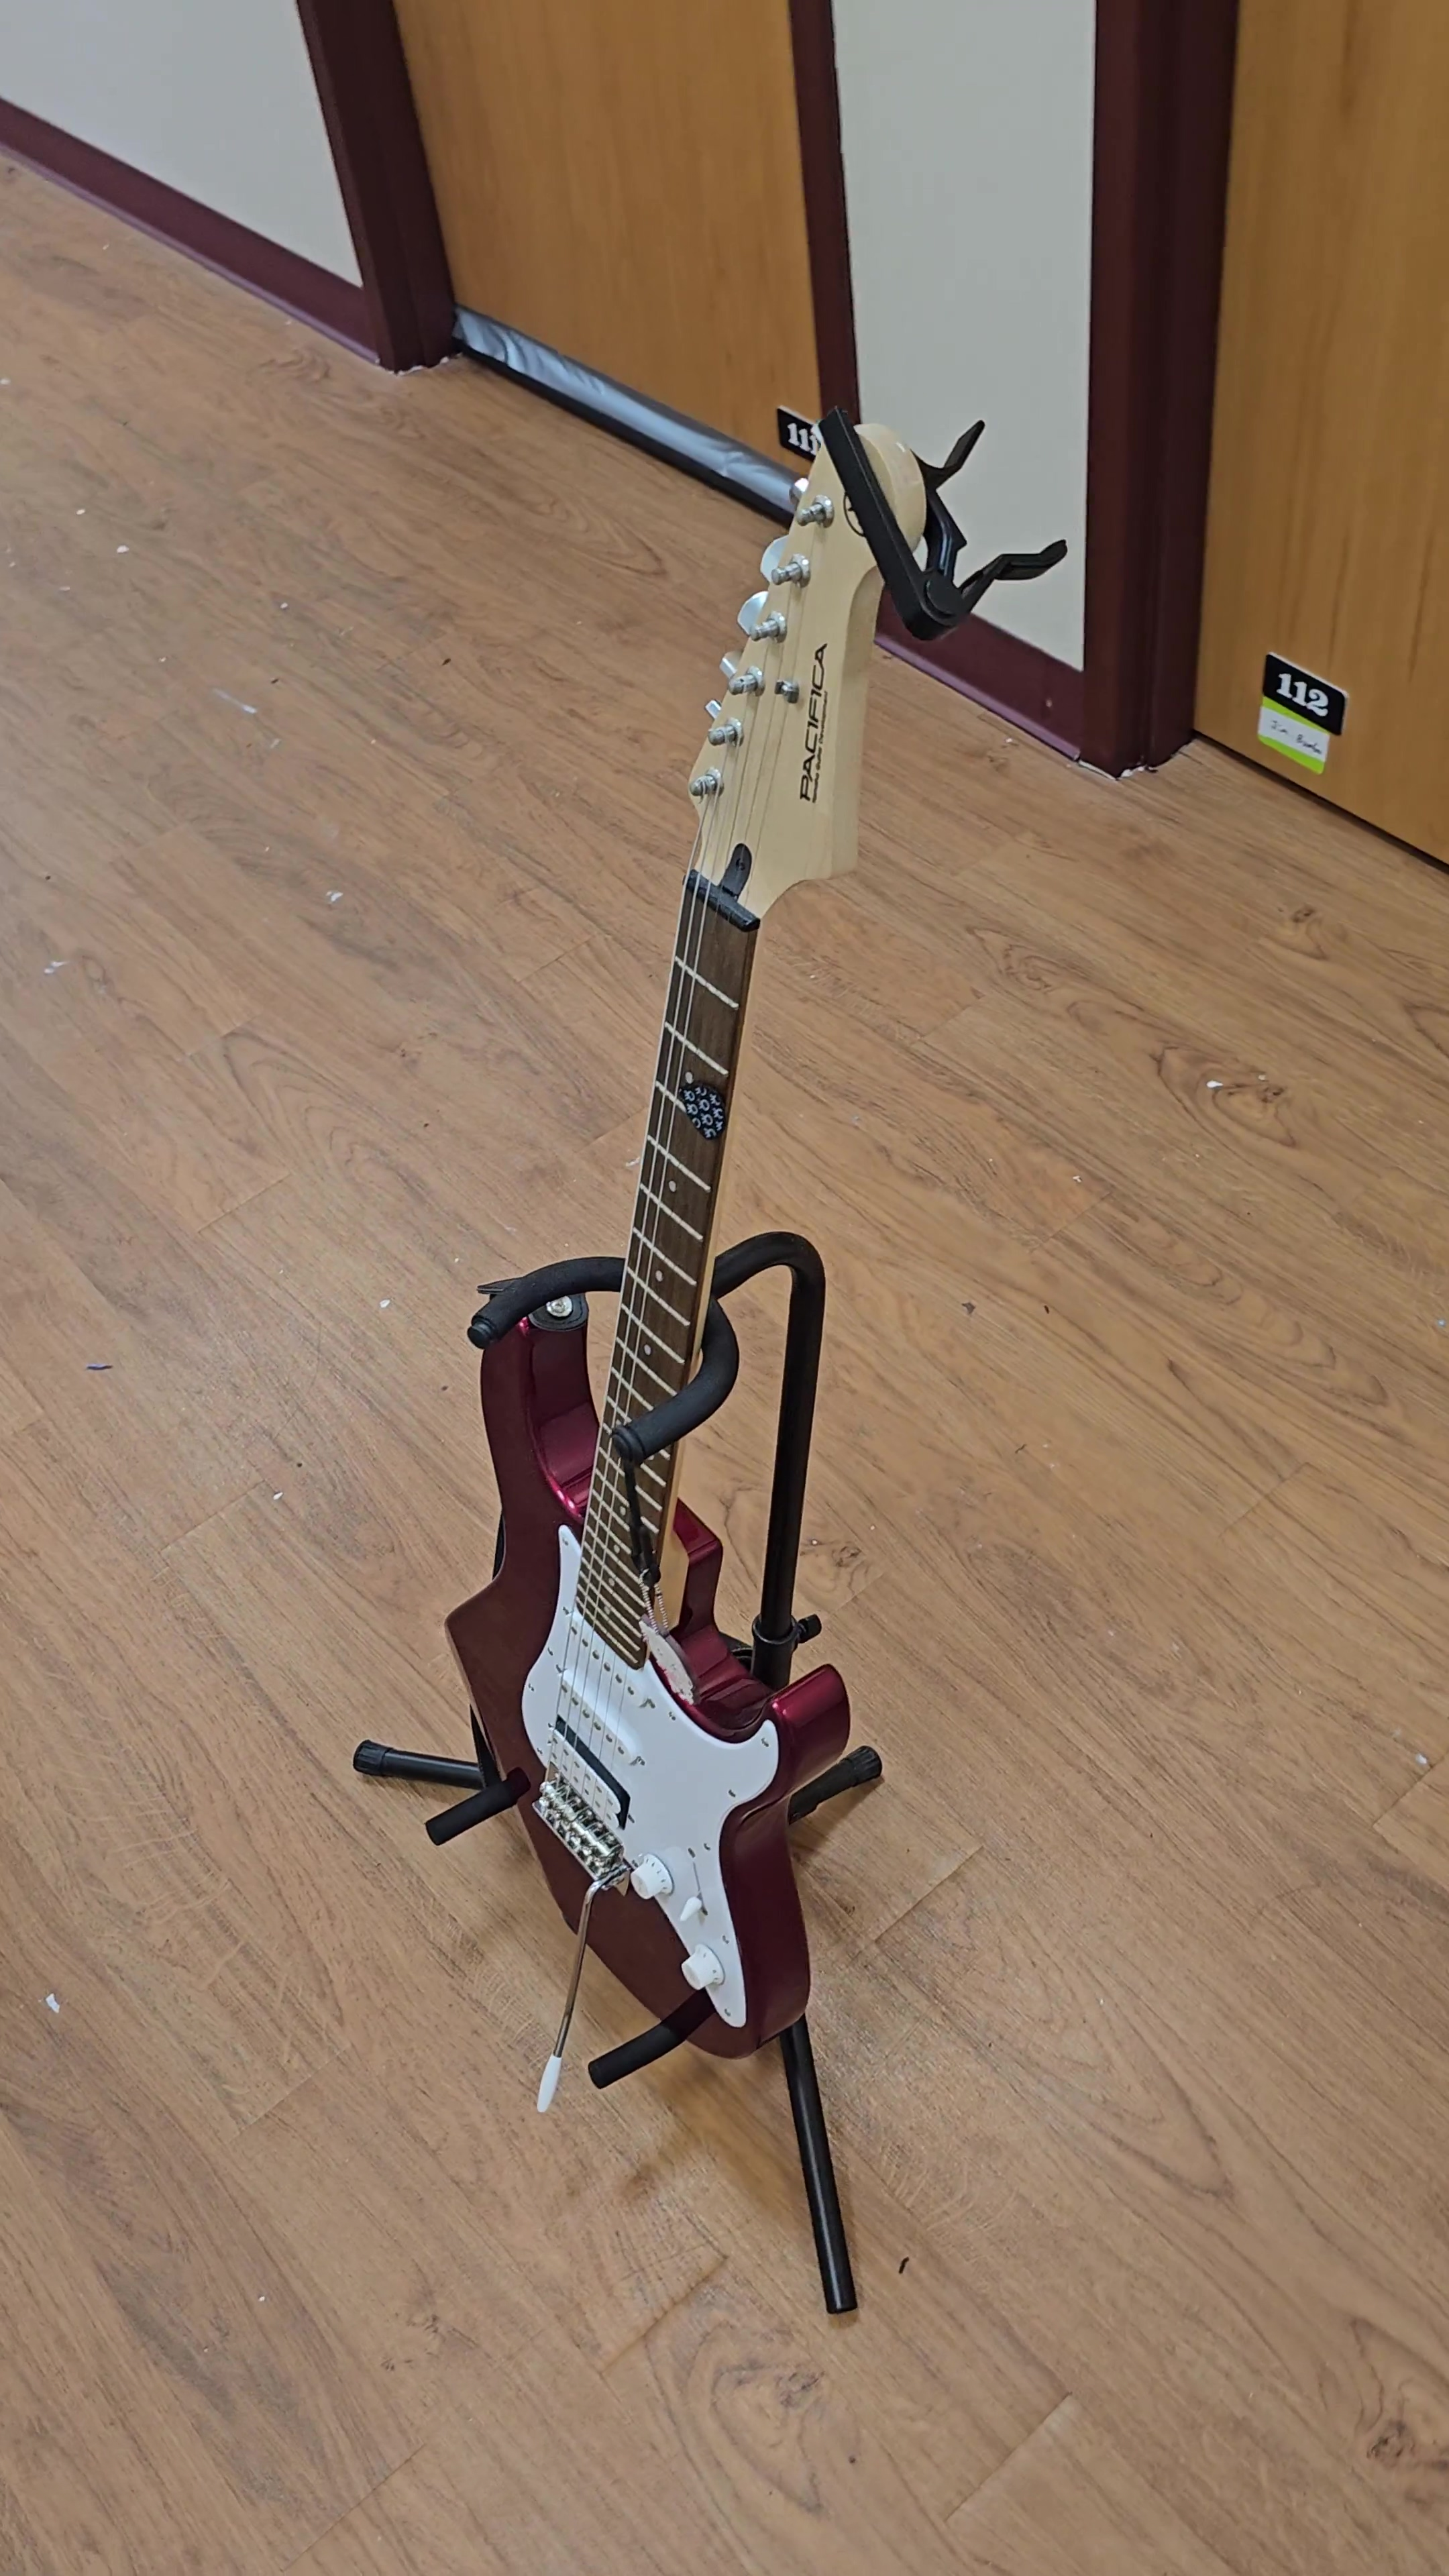
\includegraphics[scale=0.02]{images/guitar1.jpg}
    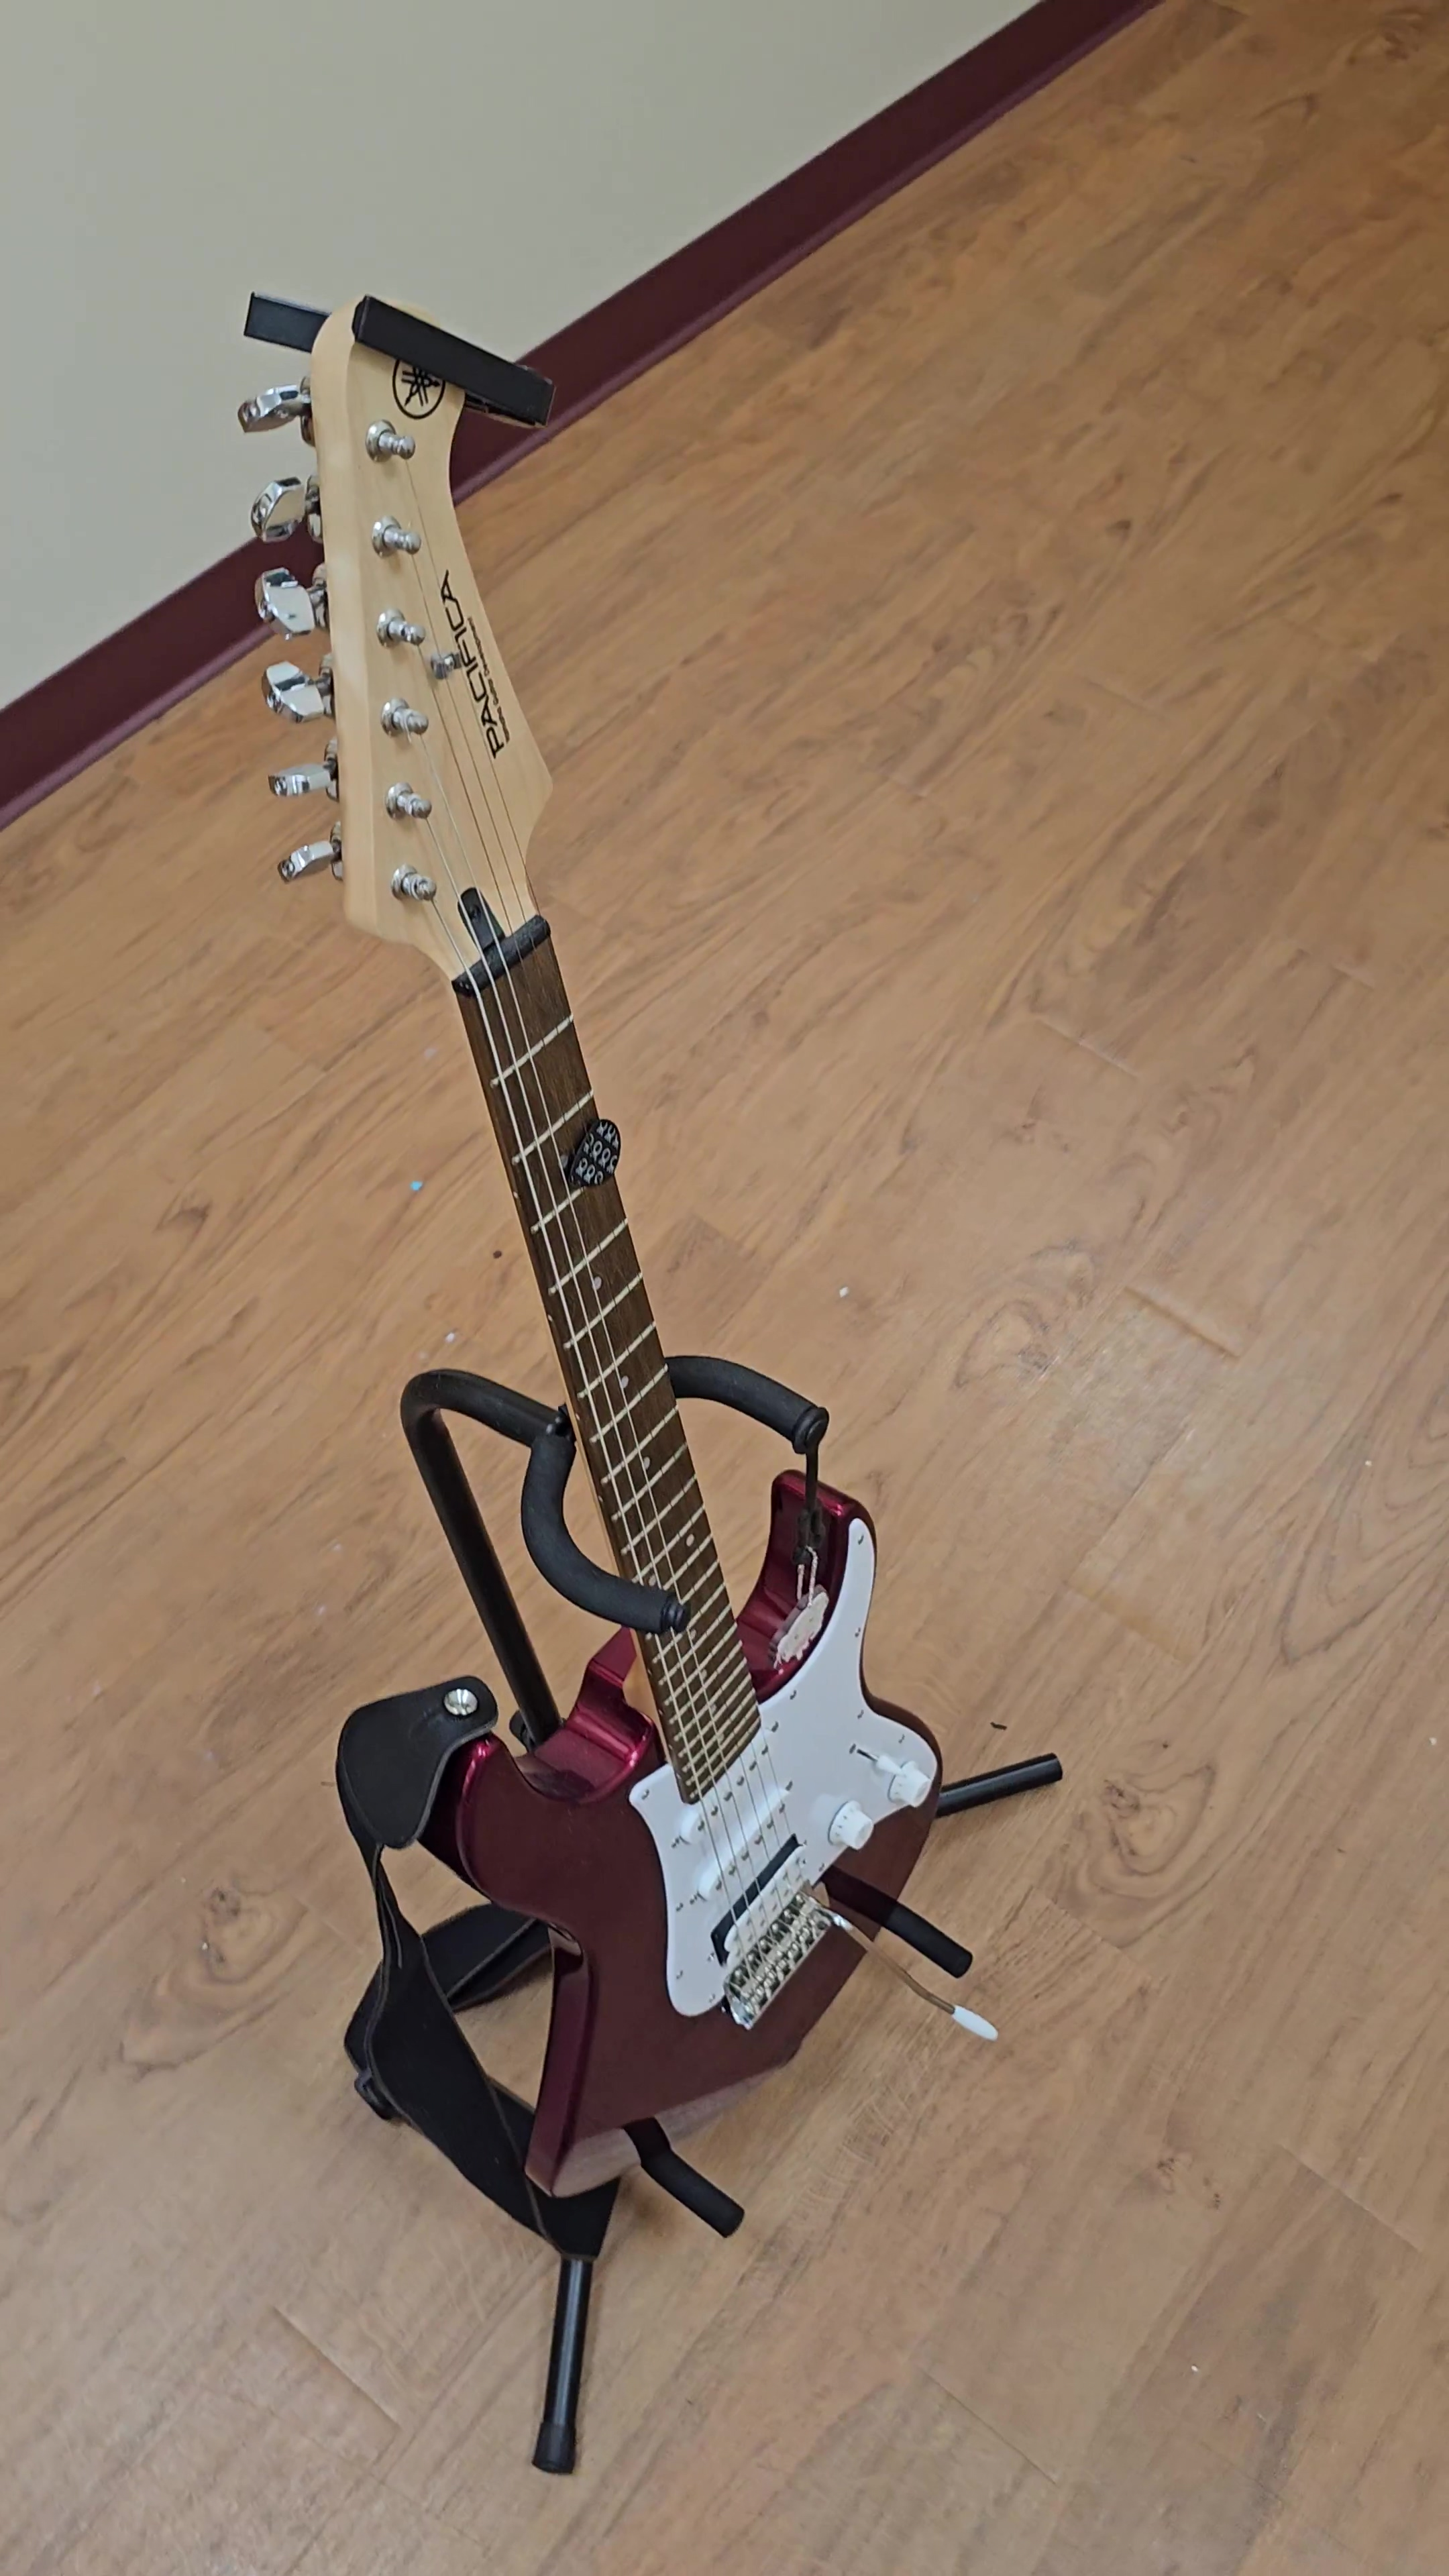
\includegraphics[scale=0.02]{images/guitar2.jpg}
    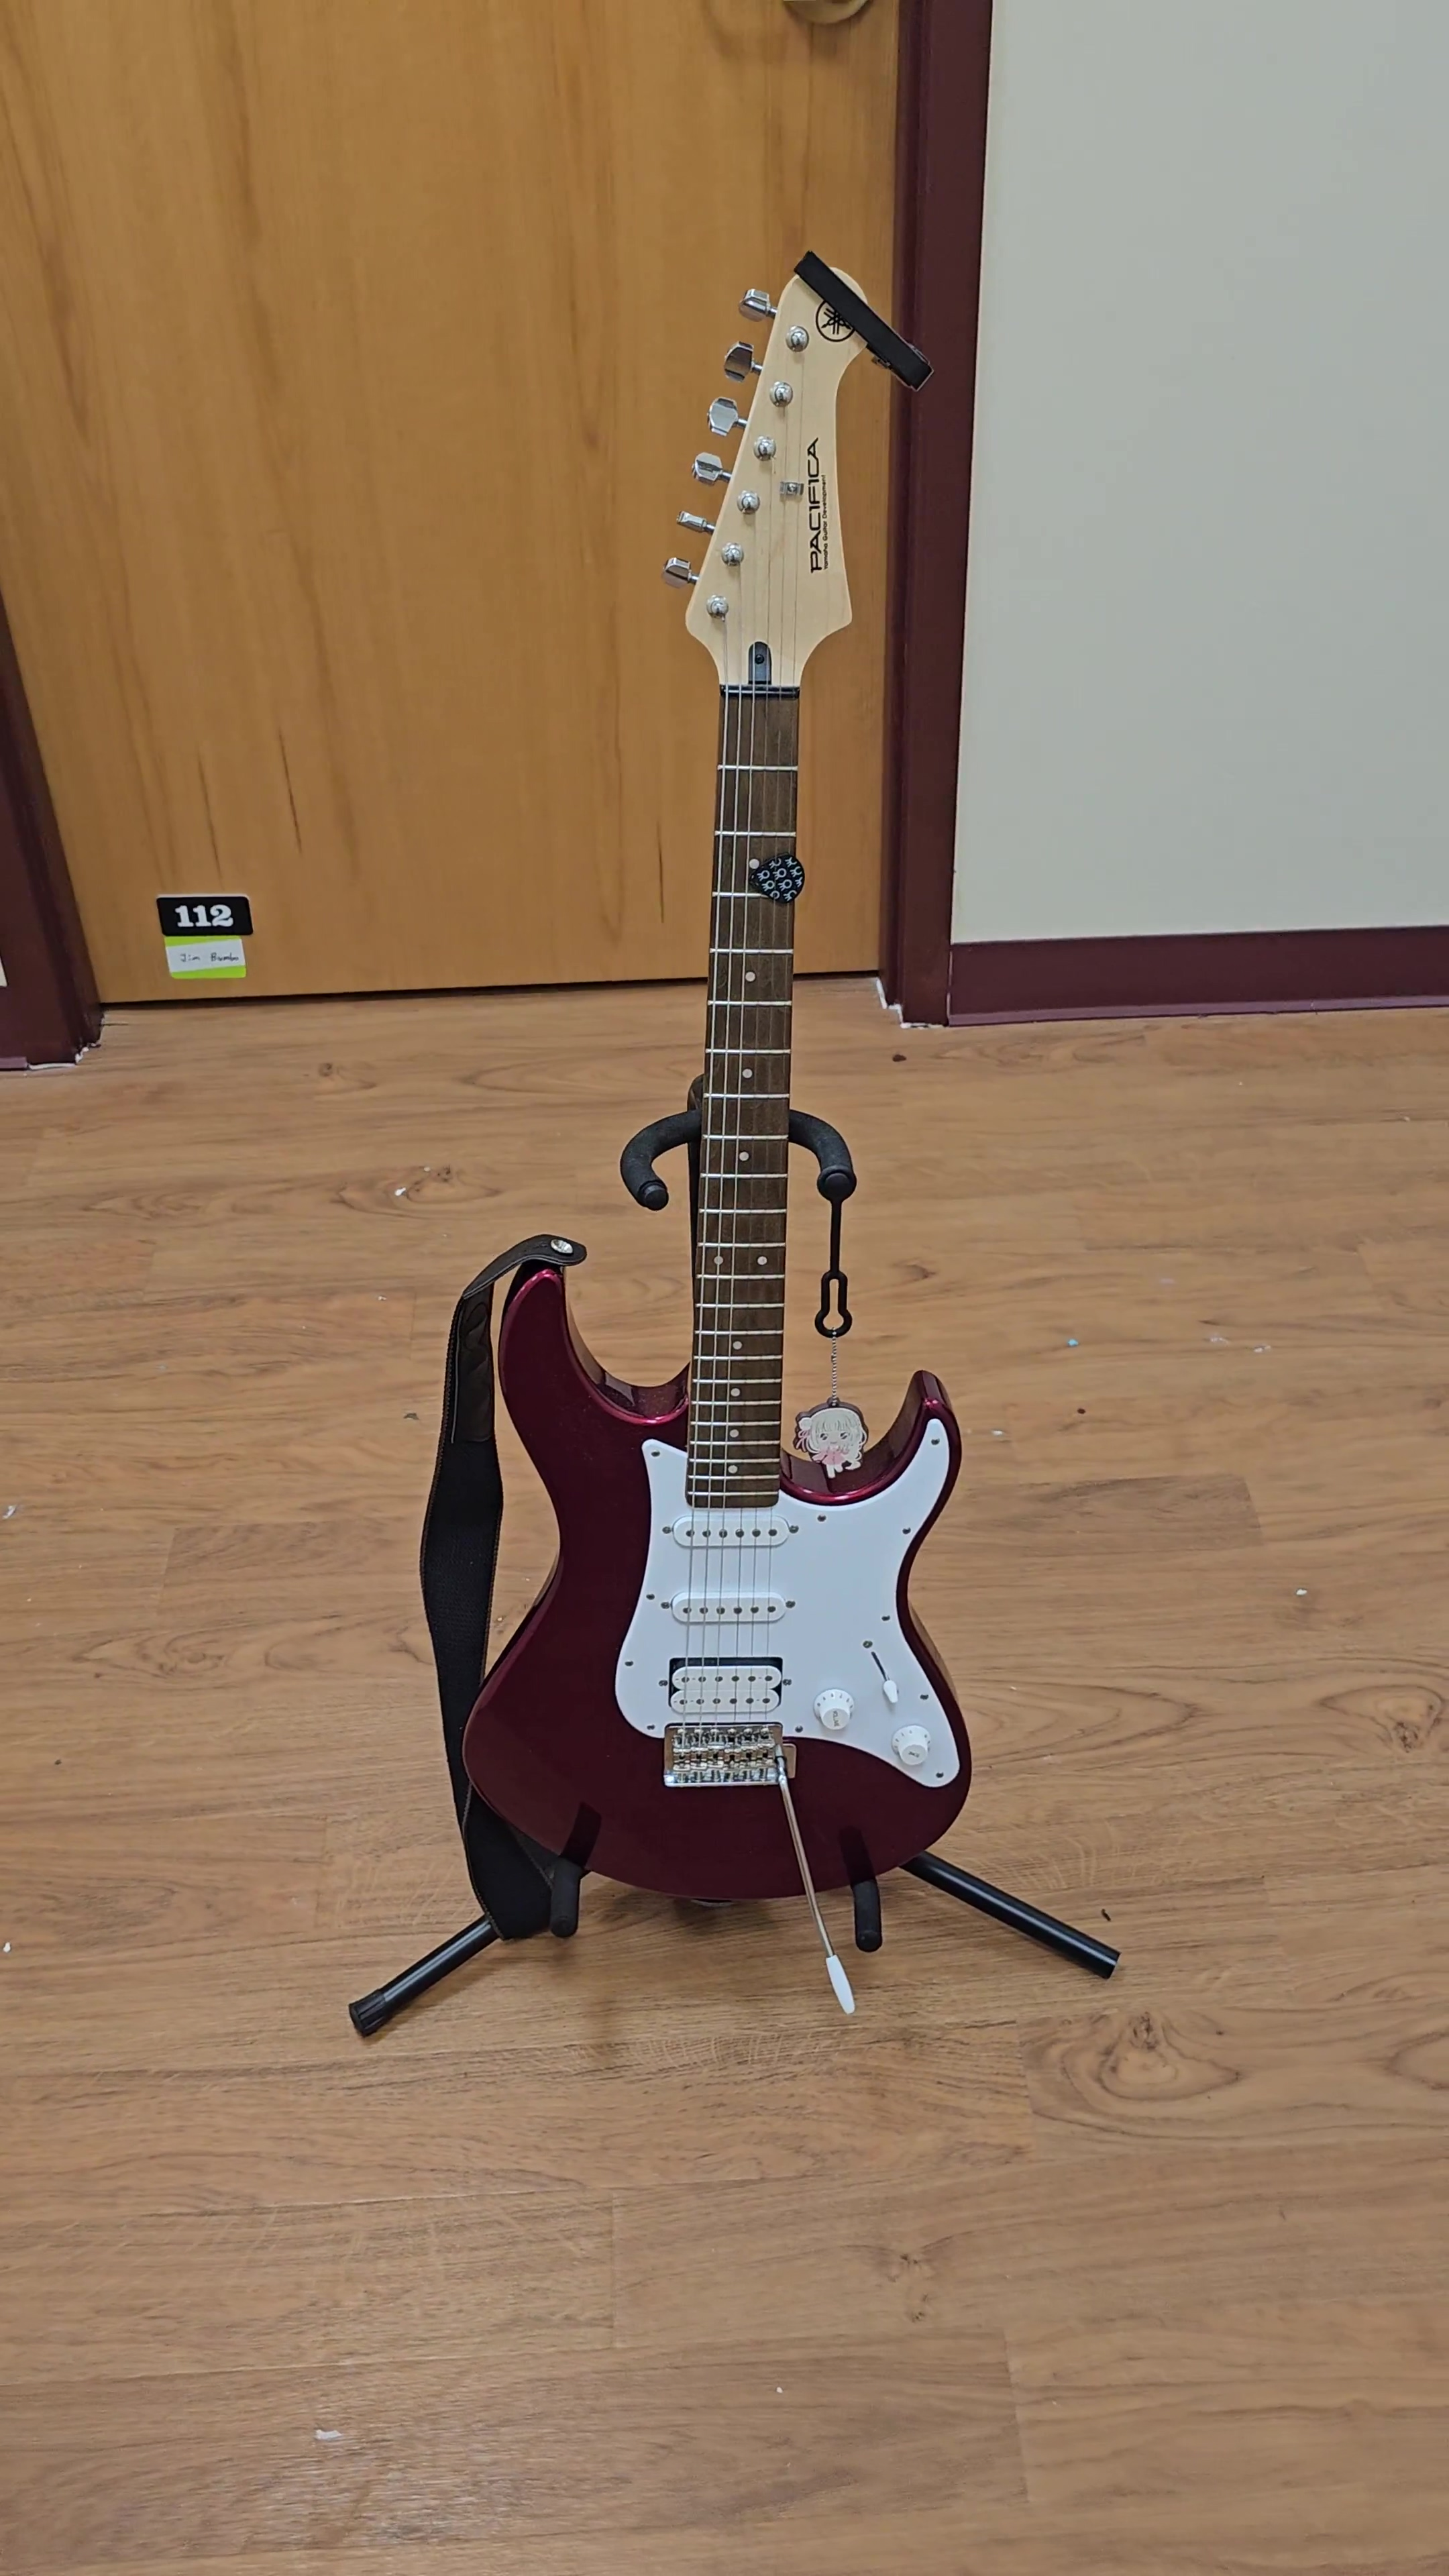
\includegraphics[scale=0.02]{images/guitar3.jpg}\\
    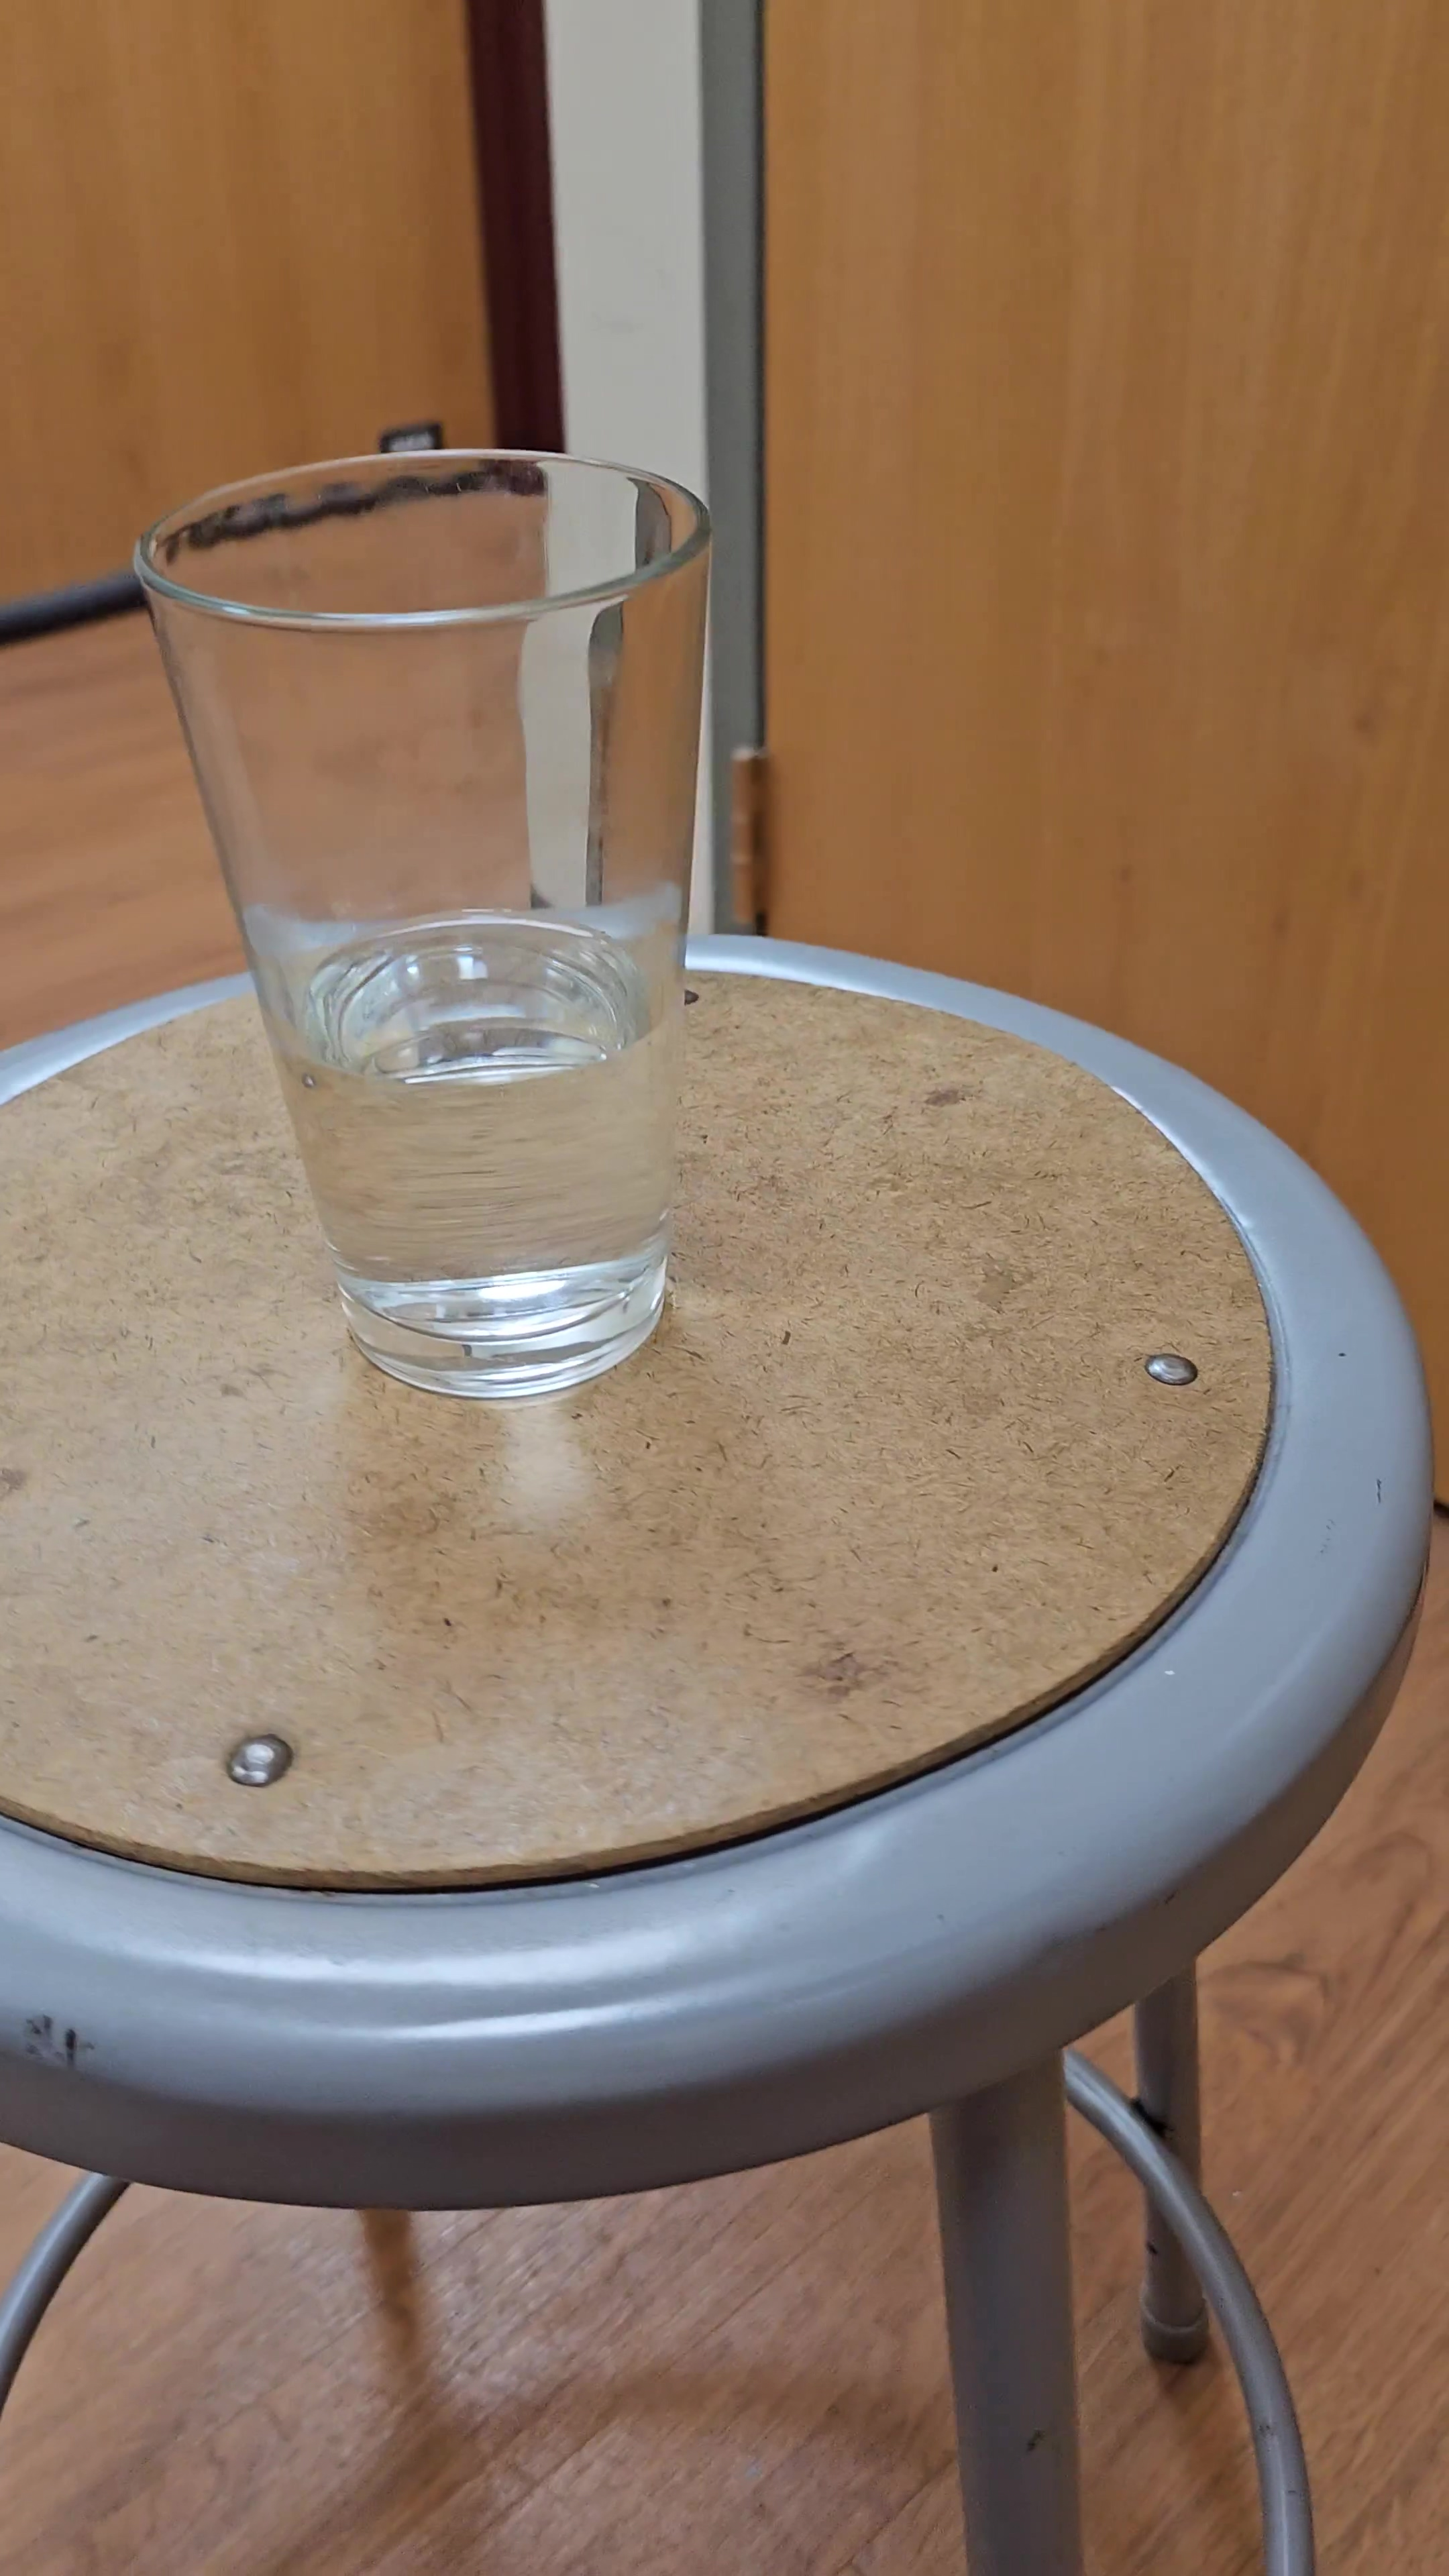
\includegraphics[scale=0.02]{images/water1.jpg}
    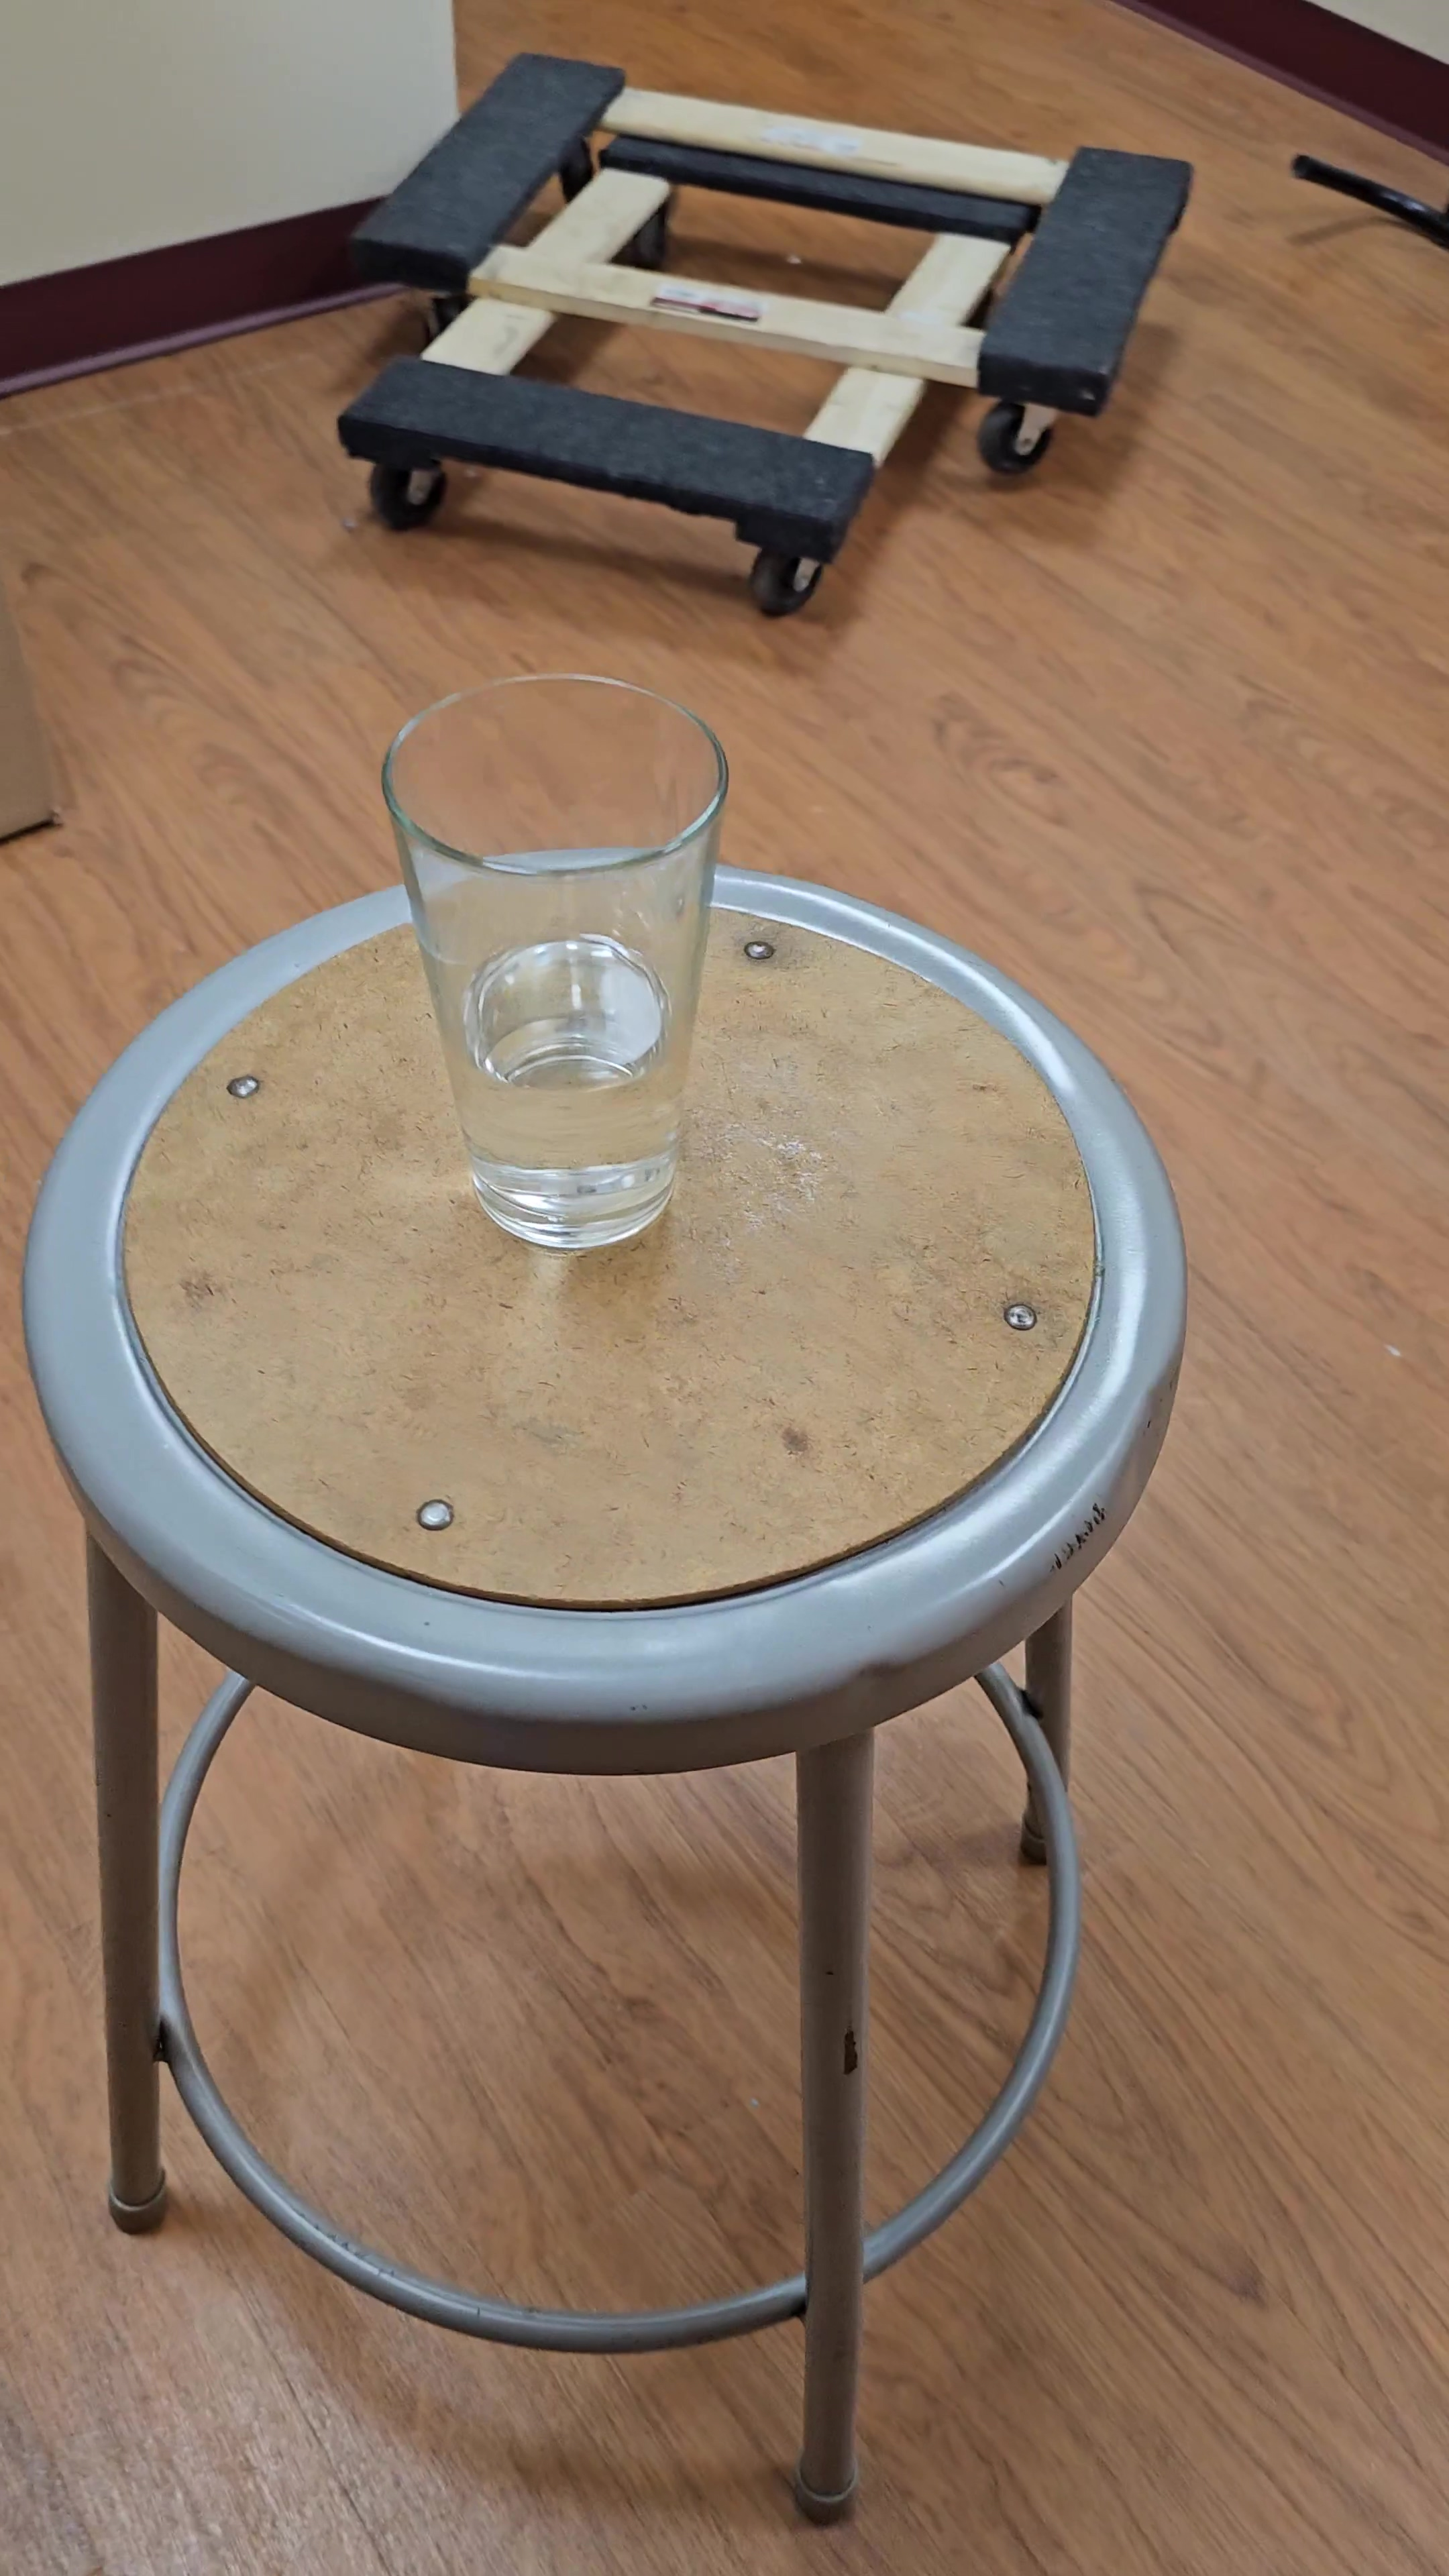
\includegraphics[scale=0.02]{images/water2.jpg}
    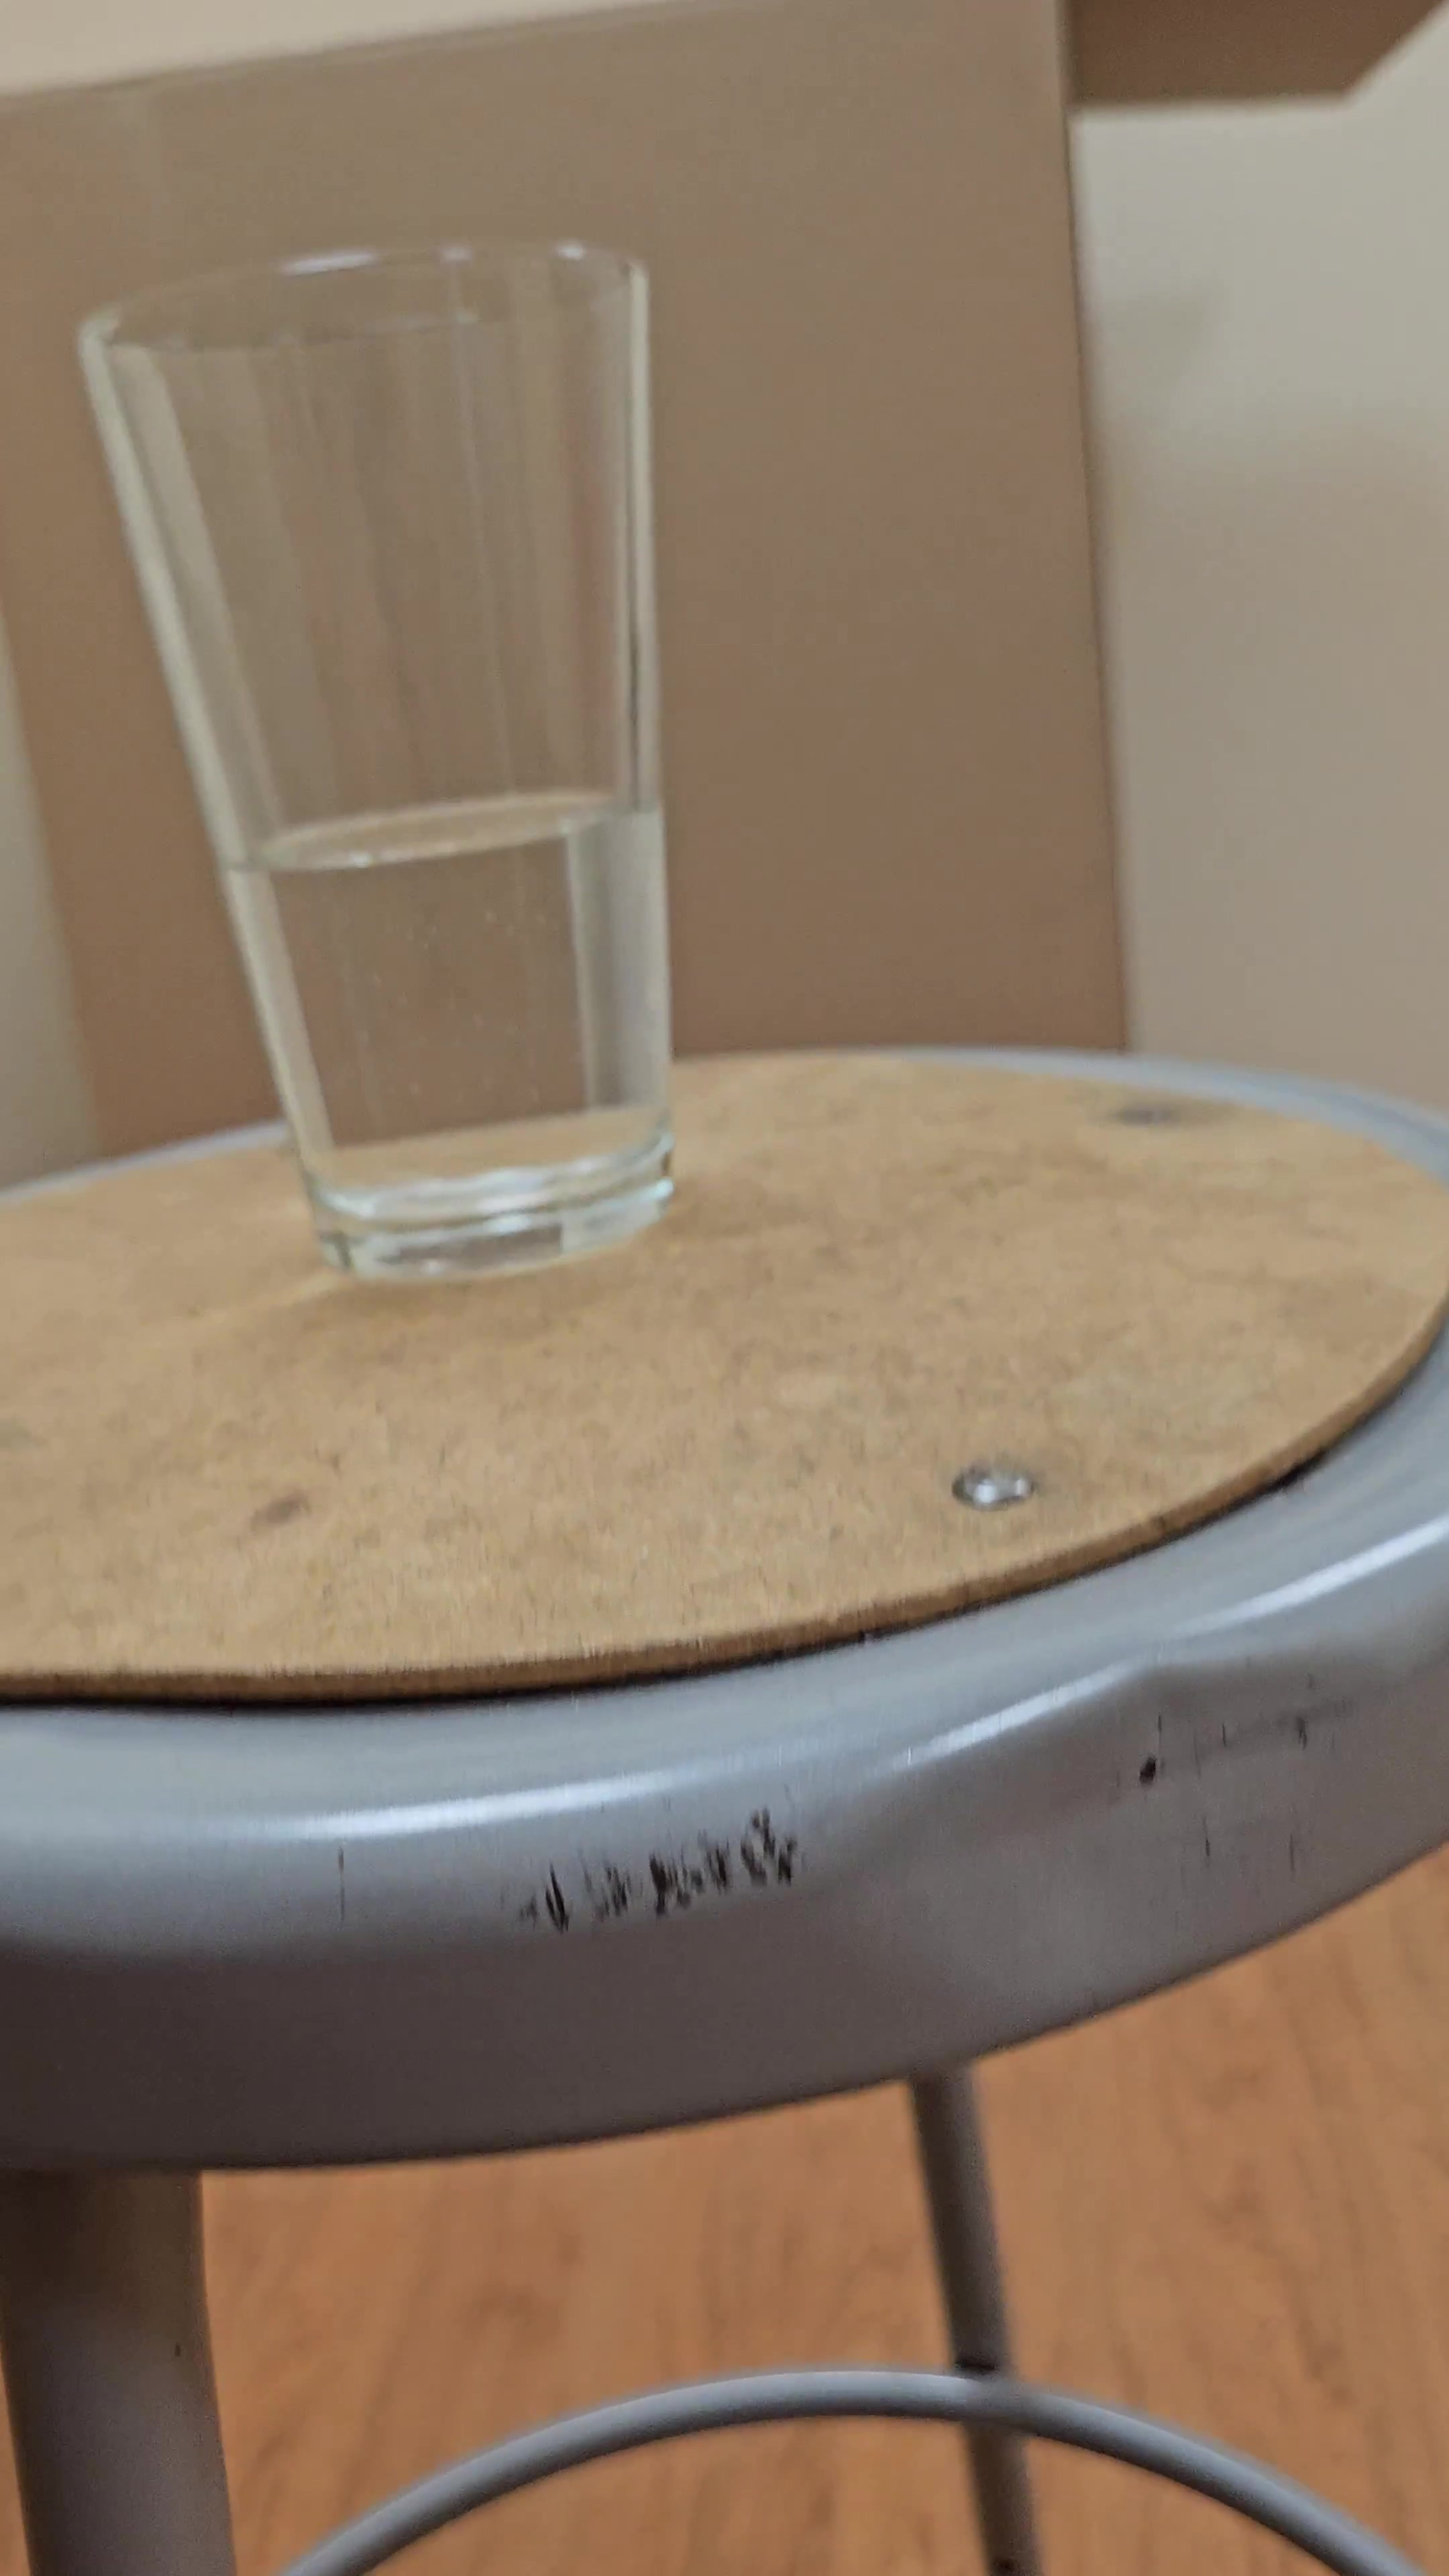
\includegraphics[scale=0.02]{images/water3.jpg}\\
    Figure 1: Dataset
\end{center}

As you can see, we want to test different objects with different refractive indices, complex objects like a guitar, and somewhat the environment around them. The videos are then transcribed into images which takes 5 frames per second and transforms those frames into 5 images. Note: we used these dataset mostly for NeRF and for testing, we noticed later on that there were some significant issues with the videos taking the images. We added some additional videos to the dataset along with the fox from the instant-ngp dataset.

\subsubsection{Colmaps}

In order to transcribe the data for it to train with NeRFs, we need to generate a Colmap as input data of spacial locations in order to process them for NeRFs. Colmaps, also known as "Collaborative Mapping", utilizes SfM (Structure from Motion) algorithms in order to infer 3D information from multiple 2D images. 

\subsection{Parameter Choice/Tuning step}

In our testing, we did not alter any of the tuning steps for training NeRF. Here is the truncated nerfacto configuration.

\begin{verbatim}
    NerfactoModelConfig(
            collider_params={'near_plane': 2.0, 'far_plane': 6.0},
            loss_coefficients={'rgb_loss_coarse': 1.0, 'rgb_loss_fine': 1.0},
            eval_num_rays_per_chunk=32768,
            near_plane=0.05,
            far_plane=1000.0,
            hidden_dim=64,
            hidden_dim_color=64,
            hidden_dim_transient=64,
            num_levels=16,
            base_res=16,
            max_res=2048,
            log2_hashmap_size=19,
            features_per_level=2,
            num_proposal_samples_per_ray=(256, 96),
            num_nerf_samples_per_ray=48,
            num_proposal_iterations=2,
            proposal_initial_sampler='piecewise',
            interlevel_loss_mult=1.0,
            distortion_loss_mult=0.002,
            orientation_loss_mult=0.0001,
            pred_normal_loss_mult=0.001,
            implementation='tcnn',
            appearance_embed_dim=32)
\end{verbatim}

\subsection{Nerfstudio}

In order to train our data, we utilized nerfstudio, an API that provided the process of creating NeRFs, loading in NeRF models and support for other tools. The Nerfstudio developed a "defacto" method of NeRF that combines other methods of NeRF models that generally worked well. Unfortunately the only information of this model is defined on their documentation.

\subsubsection{Nerfacto}
\begin{center}
    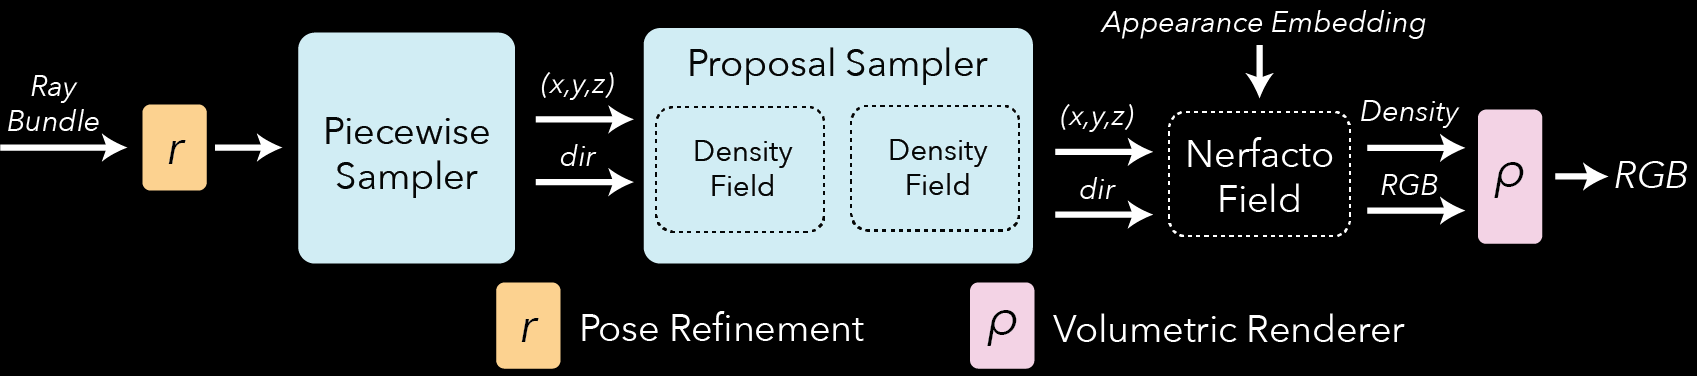
\includegraphics[scale=0.2]{models_nerfacto_pipeline.png}
\end{center}
Before the data is even sent to the neural radiance field, the pipeline performs some data preprocessing that assists the model. If we examine the dataset that is taken by humans, especially through mobile devices, notice that the movement of the camera is not always smooth and there will be artifacts in generalizing a field. This leads to problems when the NeRF generates artifacts around images and causing loss in detail, since it was unable to predict the correct camera pose. Therefore, in this step, when NeRF backpropagates for loss in order to find the input pose, we use that calculation to optimize the camera pose. This is a general and popular technique used for NeRFs known as "Camera pose refinement."

Afterwards, those inputs are sent to two different samplers. The first sampler, piece-wise sampler, generates two general samples of data: a uniformly distributed samples from the origin to the camera, and a larger step size of samples away. This allows for a more dense sample set for objects that are closer to the camera. Then a proposal sampler takes those samples and attempting to focus sample locations on more important areas of the scene. They is done by utilizing different density functions. Finally, the samples are sent to the neural radiance field to generate the density and color for the field.

\begin{center}
    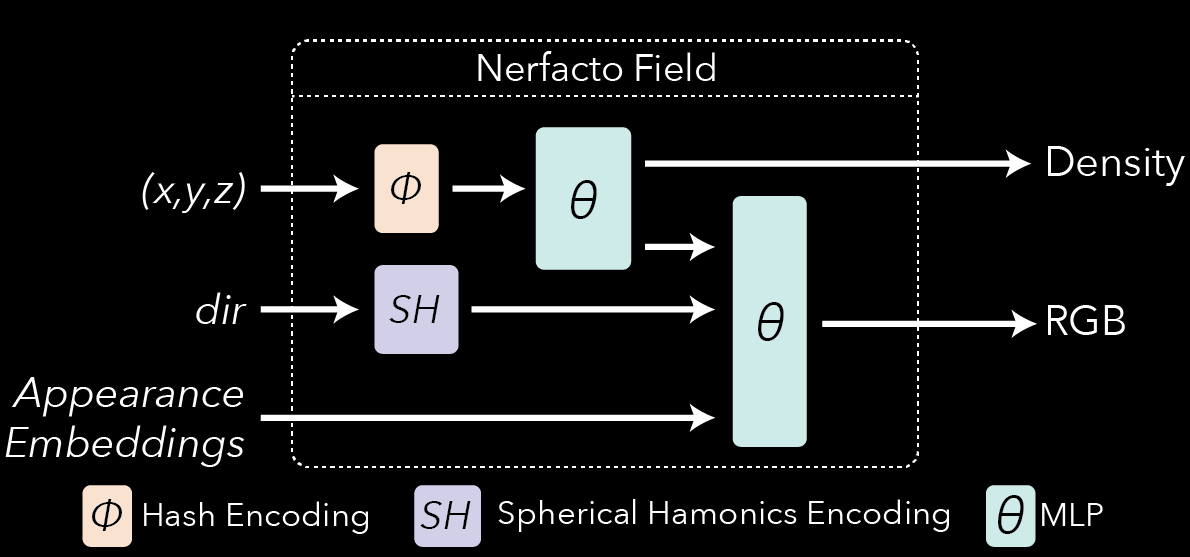
\includegraphics[scale=0.25]{models_nerfacto_field.png}
\end{center}

Like NeRF, nerfacto takes spacial coordinates the the direction vector as an input and outputs the density and color. However, in this model, the spacial location is hashed instead of a positional encoding and we use a spherical harmonics encoding with an appearance embeddings to the MLP for color. The MLP is trained and rendered with the hash input encoding with the "tiny-cuda-nn" framework.

\subsection{Reflection}

There were many issues with dependencies for colmaps, and installing correctly. Through the Microsoft vkpkg repository that has colmaps, the build fails for windows and apparently only works through linux for conda-forge. Thus, if you use NeRF studio for instruct nerf2nerf or nerfacto, then consider not using Windows unless they fix the issue or bug (since it still is an open issue on that repository). If you look at the results for certain NeRFs, you might see that some parts are more noisy than others. This is due to the fact that we did not capture a full 360 image for that specific dataset. For instance, the chair had some issues where the classroom behind it was not captured. For the glass of water on the stool, most of the image is close up, so the surrounding image of it had not been captured nicely. Thus, when capturing data/images for NeRF, there are plenty of decisions behind trying to either capture the entire scene or capture the object of that image moreso. In our case, we tried mostly to capture the object, so the scene around that object may look a bit noisy. 

For nerfstudio, using nerfacto took us 30,000 iterations in around 10 minutes to train the default model. Rendering the video with the camera paths took us around 5 minutes.

\section{NeRF Transformations: InstructNeRF2NeRF}

InstructNeRF2NeRF utilizes a diffusion model in order to edit NeRF scenes with given prompts. We were able to take a NeRF scene that was trained through nerfstudio and apply an extension to Nerfstudio that uses InstructNeRF2NeRF. This allowed us to experiment with changing the objects or items in the scene with a different item as well as try to change the environment around as well. For instance, if we have a cup of water, we want to use this framework to try and change that cup of water into a cup of milk.
% \begin{tcbraster}[raster columns=2,raster equal height,nobeforeafter,raster column skip=2cm]
%   \begin{tcolorbox}[title=box 1]
%     \lipsum[2]
%   \end{tcolorbox}
%   \begin{tcolorbox}[title=box 2]
%     \lipsum[2]
%   \end{tcolorbox}
% \end{tcbraster}

% \begin{center}
    \begin{tcbraster}[raster columns=2,raster equal height,raster column skip=0cm]
        \begin{tcolorbox}[
                          boxsep=0pt,
                          top=2pt,
                          left=4pt,
                          right=4pt,
                          colback=black!5!white,
                          colframe=black!75!black,
                          center title,
                          title=Original Picture
                          ]
            \begin{center}
                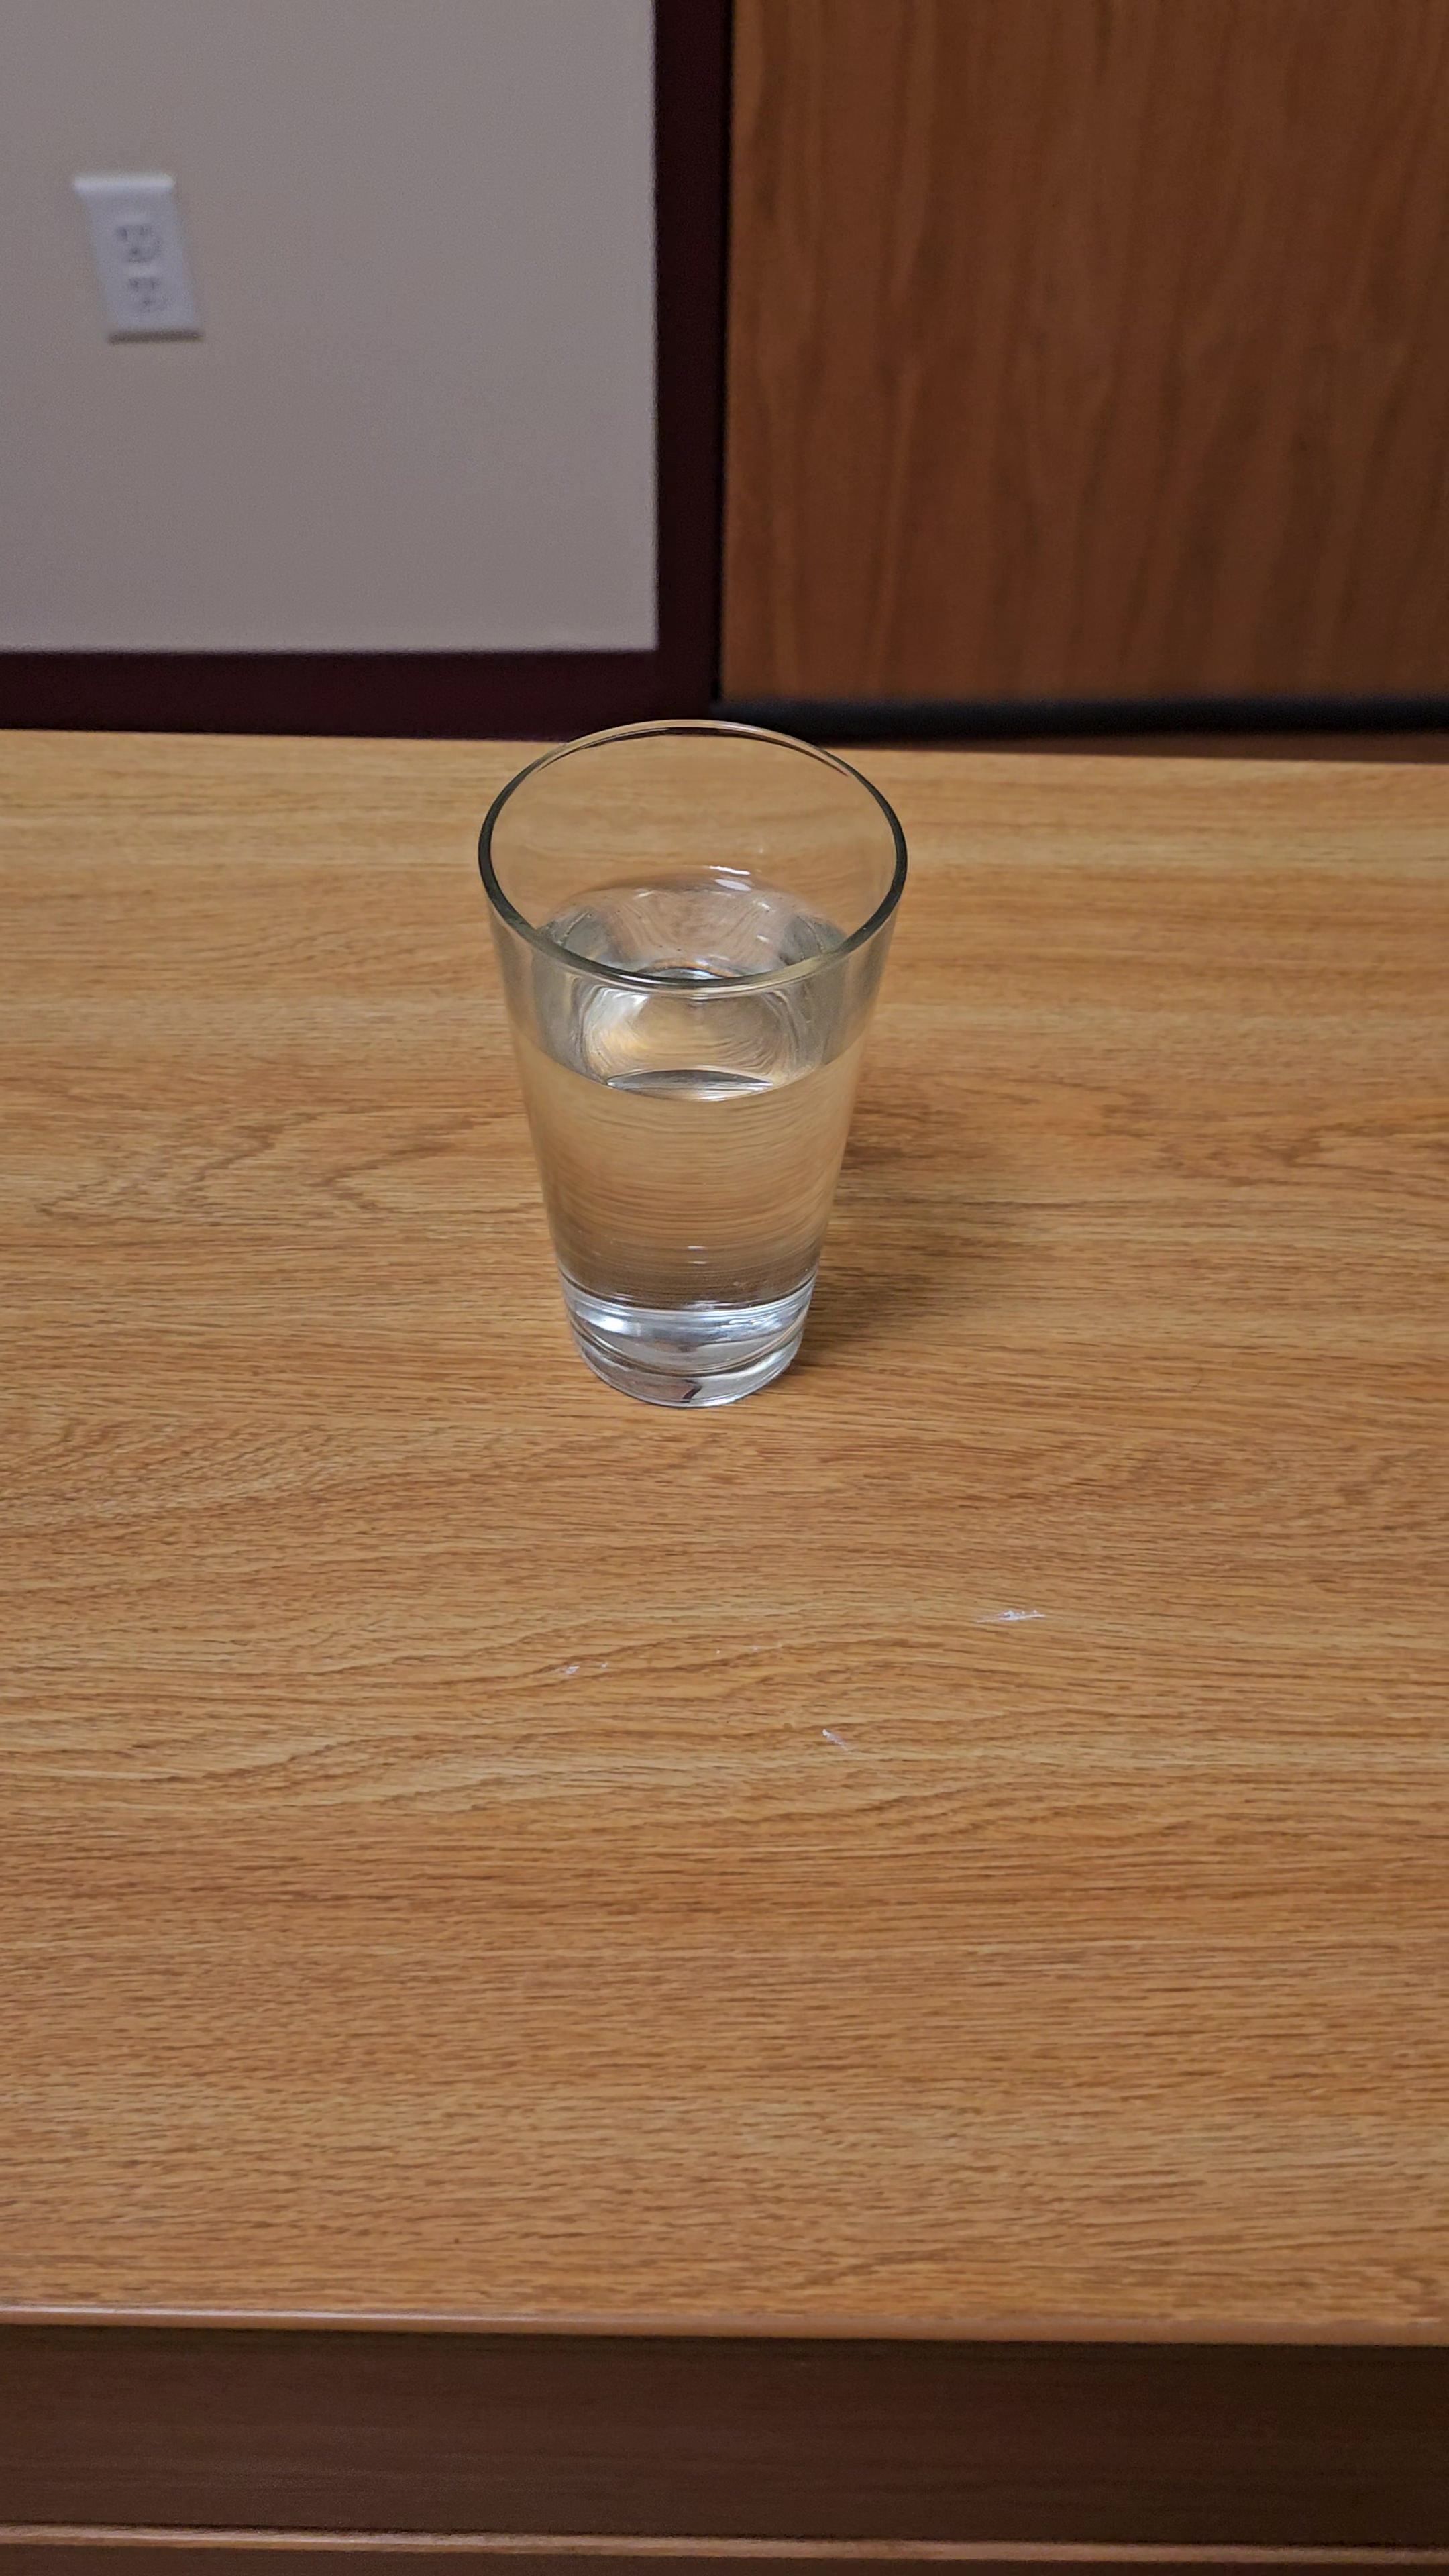
\includegraphics[scale=0.035]{images/waterinit.jpg}
            \end{center}
        \end{tcolorbox}
        \begin{tcolorbox}[
                          boxsep=0pt,
                          top=2pt,
                          left=4pt,
                          right=4pt,
                          colback=red!5!white,
                          colframe=red!75!black,
                          center title,
                          title=transform the water into milk
                          ]
        \begin{center}
            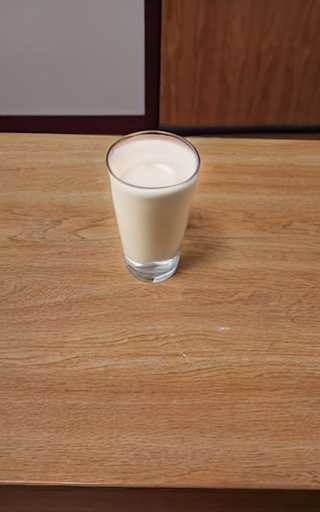
\includegraphics[scale=0.25]{images/milktransform.png}
        \end{center}
        \end{tcolorbox}
    \end{tcbraster}
% \end{center}

\section{Discussion}

% In retrospect, we tried using two different NeRF methods, 
If we examine our results, we have varying levels of success with mostly failures for InstructNeRF2NeRF. For all of the NeRF examples, especially the glass water in the cup, we can see that the refraction of the water in the cup actually matches very well with the scene in the result. Moreover, in our other scenes, we can see that it generalizes the scene very well based on the data that is captured for it. Therefore, we can claim that our NeRF models were successful with nerfacto. 

Through our research, InstructNeRF2NeRF utilizes InstructPix2Pix in order to generate images, and it is recommended that if our prompt works for InstructPix2Pix then it would work well for InstructNeRF2NeRF: (in this case we did not use the "glass of wine" prompt since many results did not turn out well for pix2pix).

\begin{center}
    \begin{tcolorbox}[
                      boxsep=0pt,
                      top=2pt,
                      colback=red!5!white,
                      colframe=red!75!black,
                      center title,
                      autowidth title=transform the water into milk
                      ]
        \begin{center}
            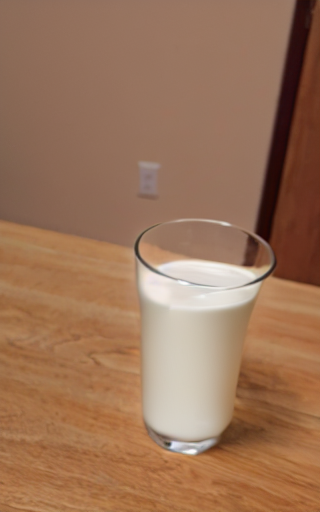
\includegraphics[scale=0.15]{images/milk.png}
        \end{center}
    \end{tcolorbox}

    \begin{tcolorbox}[
                      boxsep=0pt,
                      top=2pt,
                      colback=red!5!white,
                      colframe=red!75!black,
                      center title,
                      autowidth title=turn the cup into a glass of wine
                      ]
        \begin{center}
            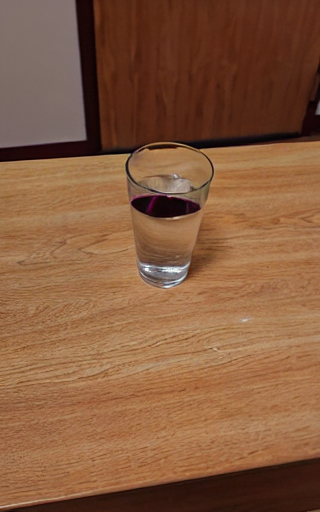
\includegraphics[scale=0.15]{images/wine.png}
        \end{center}
    \end{tcolorbox}
\end{center}
\begin{center}
    \begin{tcolorbox}
        \textbf{ To easily differentiate between InstructPix2Pix and InstructNeRF2NeRF, a red box will be used for Pix2Pix results while a blue box will be used for NeRF2NeRF results. }
    \end{tcolorbox}
\end{center}

\newpage
There were certain prompts that did not have good results. For instance, animals that are closer to each other than others have higher similarities and in respect to that, looks much closer to each other. In the example below, note that the wolf looks very good, meanwhile the dog could need some work with that makeup.

\begin{center}
    \begin{tcolorbox}[
                      boxsep=0pt,
                      top=2pt,
                      colback=red!5!white,
                      colframe=red!75!black,
                      center title,
                      autowidth title=turn the fox into a wolf
                      ]
        \begin{center}
            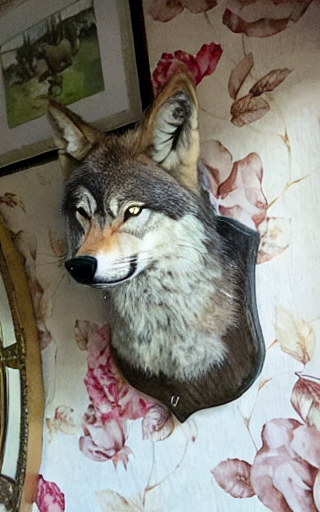
\includegraphics[scale=0.15]{images/wolf.png}
        \end{center}
    \end{tcolorbox}
    \begin{tcolorbox}[
                      boxsep=0pt,
                      top=2pt,
                      colback=red!5!white,
                      colframe=red!75!black,
                      center title,
                      autowidth title=turn the fox into a dog
                      ]
        \begin{center}
            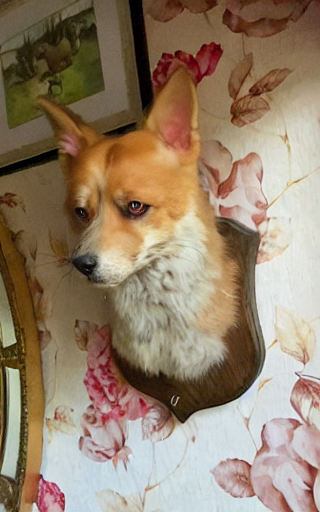
\includegraphics[scale=0.15]{images/dog.png}
        \end{center}
    \end{tcolorbox}
\end{center}

However, in general, most results for InstructNeRF2NeRF did not work well as intended. Although we are uncertain about the exact reasoning why, we might have several indications of why this might be the case. Previously, we mentioned that InstructNeRF2NeRF takes InstructPix2Pix over the NeRF scene. Thus, certain cases worked well and some didn't for InstructPix2Pix. However, since InstructPix2Pix is applied to different images over time, there can be large inconsistencies between the images generated between the datapoints. Thus, the result for the NeRF will attempt to go inbetween and result in some errors. For example, for one image it can generate orange juice perfectly, but for the other image it can generate orange juice, but add random oranges in the background (throwing everything off).

\begin{center}
    \begin{tcolorbox}[
                      boxsep=0pt,
                      top=2pt,
                      colback=red!5!white,
                      colframe=red!75!black,
                      center title,
                      autowidth title=turn the water to orange juice
                      ]
        \begin{center}
            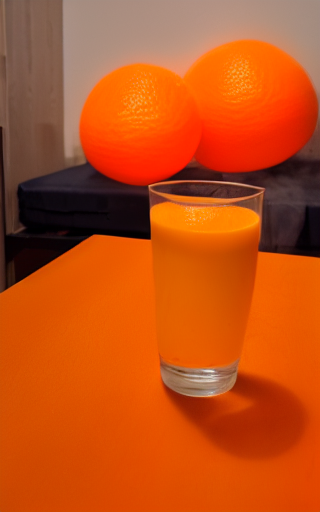
\includegraphics[scale=0.2]{images/orangejuicefail.png}
        \end{center}
    \end{tcolorbox}
\end{center}

Moreover, there are certain cases where we have a working example for InstructPix2Pix, but the result for InstructNeRF2NeRF did not look as precise as the result from Pix2Pix.

\begin{center}
    \begin{tcolorbox}[
                      boxsep=0pt,
                      top=2pt,
                      colback=red!5!white,
                      colframe=red!75!black,
                      center title,
                      autowidth title=turn the water to a red solo cup
                      ]
        \begin{center}
            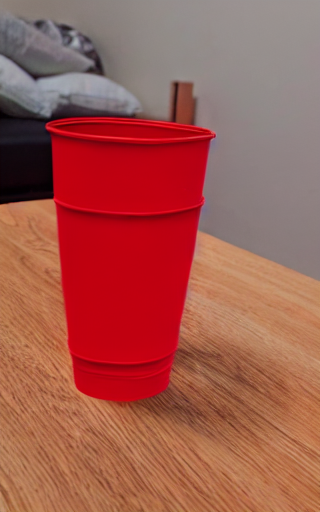
\includegraphics[scale=0.15]{images/redsolocup.png}
        \end{center}
    \end{tcolorbox}
    \begin{tcolorbox}[
                      hbox,
                      boxsep=0pt,
                      left=4pt,
                      right=4pt,
                      top=2pt,
                      colback=blue!5!white,
                      colframe=blue!75!black,
                      center title,
                      autowidth title=turn the water to a red solo cup
                      ]
            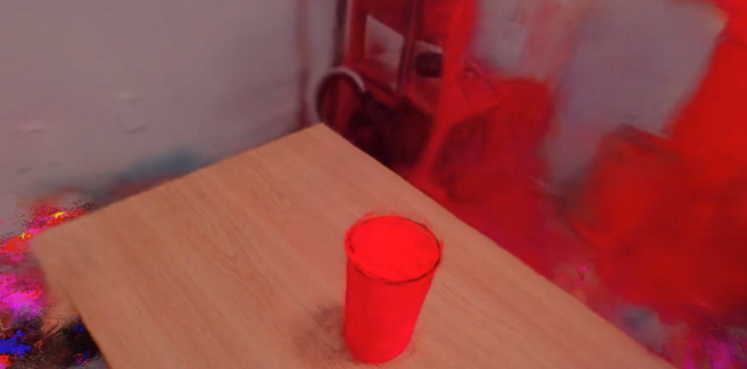
\includegraphics[scale=0.5]{images/resultcup.png}
    \end{tcolorbox}
    \begin{tcolorbox}
        At least for this example, the glass is a red cup. However, most of the room transformed to red. This can be a cause of the diffusive steps being too high or possibly too long in training.
    \end{tcolorbox}
\end{center}

\newpage
In some instances we can see that there are certain errors with training, but early stopping can help with making a result look decent rather than terrible. In this case, we have a InstructPix2Pix example that failed. However, when we tried with InstructNeRF2NeRF it had similar results as the "red solo cup" example. That is, where the surroundings transformed into that color.

\begin{center}
    \begin{tcolorbox}[
                      boxsep=0pt,
                      top=2pt,
                      colback=red!5!white,
                      colframe=red!75!black,
                      center title,
                      autowidth title=turn the water to orange juice
                      ]
        \begin{center}
            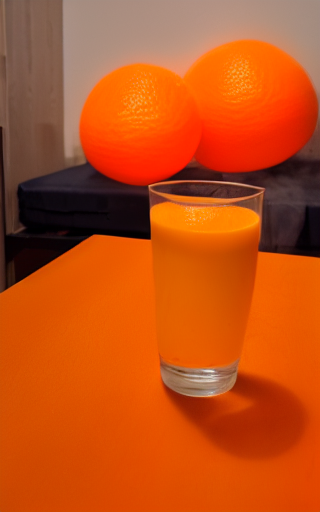
\includegraphics[scale=0.15]{images/orangejuicefail.png}
        \end{center}
    \end{tcolorbox}
    \begin{tcolorbox}[
                      hbox,
                      boxsep=0pt,
                      left=4pt,
                      right=4pt,
                      top=2pt,
                      colback=blue!5!white,
                      colframe=blue!75!black,
                      center title,
                      autowidth title=turn the water to orange juice
                      ]
            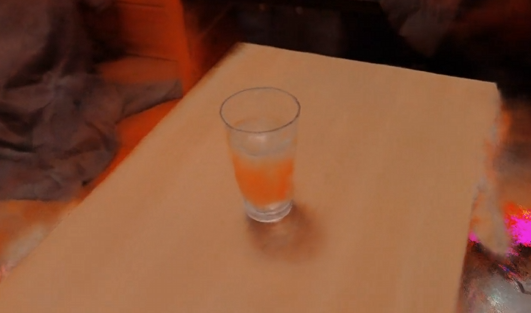
\includegraphics[scale=0.5]{images/oj.png}
    \end{tcolorbox}
\end{center}

In addition to the orange juice example, we can see that this model does not work too well with an environment that has too many different and obtuse backgrounds (with different items). The color of the background eventually bleeds in with the color of the item.

\newpage
Here is an example of InstructNeRF2NeRF working very well:
\begin{center}
    \begin{tcolorbox}[
                      width=2in,
                      boxsep=0pt,
                      top=2pt,
                      left=4pt,
                      right=4pt,
                      colback=black!5!white,
                      colframe=black!75!black,
                      center title,
                      title=Original NeRF
                      ]
        \begin{center}
            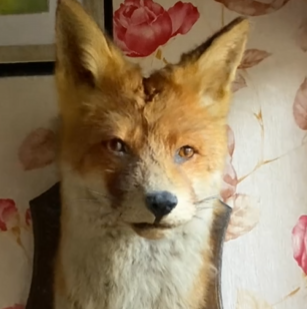
\includegraphics[scale=0.4]{images/normalfox.PNG}
        \end{center}
    \end{tcolorbox}
    \begin{tcolorbox}[
                      boxsep=0pt,
                      top=2pt,
                      colback=blue!5!white,
                      colframe=blue!75!black,
                      center title,
                      autowidth title=transform the fox into an arctic fox
                      ]
        \begin{center}
            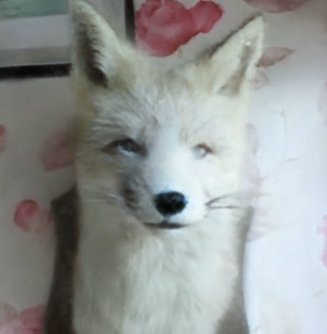
\includegraphics[scale=0.4]{images/arcticfox.PNG}
        \end{center}
    \end{tcolorbox}
    \begin{tcolorbox}[
                      boxsep=0pt,
                      left=0pt,
                      right=0pt,
                      top=2pt,
                      colback=blue!5!white,
                      colframe=blue!75!black,
                      center title,
                      autowidth title=transform the fox into a wolf
                      ]
        \begin{center}
            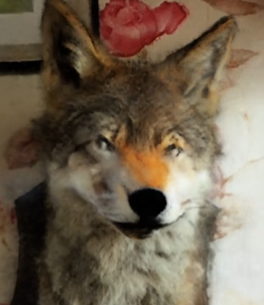
\includegraphics[scale=0.4]{images/wolfin2n.PNG}
        \end{center}
    \end{tcolorbox}
    For some reason, the nose turned more orange than the fox's nose. Perhaps, all of the fox's color got drained into the nose when transforming into a wolf.
\end{center}

\section{Resources Used}

InstructNerf2Nerf: \href{https://github.com/ayaanzhaque/instruct-nerf2nerf/tree/main#tips}{link}\\
Nerfstudio: \href{https://docs.nerf.studio}{link}\\
Instant-Ngp (for instant-ngp testing v. nerfacto): \href{https://github.com/NVlabs/instant-ngp}{link}\\
InstructPix2Pix Testing: \href{https://huggingface.co/spaces/timbrooks/instruct-pix2pix}{link}\\

\end{document}
